\documentclass[twoside]{book}

% Packages required by doxygen
\usepackage{fixltx2e}
\usepackage{calc}
\usepackage{doxygen}
\usepackage[export]{adjustbox} % also loads graphicx
\usepackage{graphicx}
\usepackage[utf8]{inputenc}
\usepackage{makeidx}
\usepackage{multicol}
\usepackage{multirow}
\PassOptionsToPackage{warn}{textcomp}
\usepackage{textcomp}
\usepackage[nointegrals]{wasysym}
\usepackage[table]{xcolor}

% Font selection
\usepackage[T1]{fontenc}
\usepackage[scaled=.90]{helvet}
\usepackage{courier}
\usepackage{amssymb}
\usepackage{sectsty}
\renewcommand{\familydefault}{\sfdefault}
\allsectionsfont{%
  \fontseries{bc}\selectfont%
  \color{darkgray}%
}
\renewcommand{\DoxyLabelFont}{%
  \fontseries{bc}\selectfont%
  \color{darkgray}%
}
\newcommand{\+}{\discretionary{\mbox{\scriptsize$\hookleftarrow$}}{}{}}

% Page & text layout
\usepackage{geometry}
\geometry{%
  a4paper,%
  top=2.5cm,%
  bottom=2.5cm,%
  left=2.5cm,%
  right=2.5cm%
}
\tolerance=750
\hfuzz=15pt
\hbadness=750
\setlength{\emergencystretch}{15pt}
\setlength{\parindent}{0cm}
\setlength{\parskip}{3ex plus 2ex minus 2ex}
\makeatletter
\renewcommand{\paragraph}{%
  \@startsection{paragraph}{4}{0ex}{-1.0ex}{1.0ex}{%
    \normalfont\normalsize\bfseries\SS@parafont%
  }%
}
\renewcommand{\subparagraph}{%
  \@startsection{subparagraph}{5}{0ex}{-1.0ex}{1.0ex}{%
    \normalfont\normalsize\bfseries\SS@subparafont%
  }%
}
\makeatother

% Headers & footers
\usepackage{fancyhdr}
\pagestyle{fancyplain}
\fancyhead[LE]{\fancyplain{}{\bfseries\thepage}}
\fancyhead[CE]{\fancyplain{}{}}
\fancyhead[RE]{\fancyplain{}{\bfseries\leftmark}}
\fancyhead[LO]{\fancyplain{}{\bfseries\rightmark}}
\fancyhead[CO]{\fancyplain{}{}}
\fancyhead[RO]{\fancyplain{}{\bfseries\thepage}}
\fancyfoot[LE]{\fancyplain{}{}}
\fancyfoot[CE]{\fancyplain{}{}}
\fancyfoot[RE]{\fancyplain{}{\bfseries\scriptsize Generated by Doxygen }}
\fancyfoot[LO]{\fancyplain{}{\bfseries\scriptsize Generated by Doxygen }}
\fancyfoot[CO]{\fancyplain{}{}}
\fancyfoot[RO]{\fancyplain{}{}}
\renewcommand{\footrulewidth}{0.4pt}
\renewcommand{\chaptermark}[1]{%
  \markboth{#1}{}%
}
\renewcommand{\sectionmark}[1]{%
  \markright{\thesection\ #1}%
}

% Indices & bibliography
\usepackage{natbib}
\usepackage[titles]{tocloft}
\setcounter{tocdepth}{3}
\setcounter{secnumdepth}{5}
\makeindex

% Hyperlinks (required, but should be loaded last)
\usepackage{ifpdf}
\ifpdf
  \usepackage[pdftex,pagebackref=true]{hyperref}
\else
  \usepackage[ps2pdf,pagebackref=true]{hyperref}
\fi
\hypersetup{%
  colorlinks=true,%
  linkcolor=blue,%
  citecolor=blue,%
  unicode%
}

% Custom commands
\newcommand{\clearemptydoublepage}{%
  \newpage{\pagestyle{empty}\cleardoublepage}%
}

\usepackage{caption}
\captionsetup{labelsep=space,justification=centering,font={bf},singlelinecheck=off,skip=4pt,position=top}

%===== C O N T E N T S =====

\begin{document}

% Titlepage & ToC
\hypersetup{pageanchor=false,
             bookmarksnumbered=true,
             pdfencoding=unicode
            }
\pagenumbering{alph}
\begin{titlepage}
\vspace*{7cm}
\begin{center}%
{\Large Matrix\+Engine }\\
\vspace*{1cm}
{\large Generated by Doxygen 1.8.13}\\
\end{center}
\end{titlepage}
\clearemptydoublepage
\pagenumbering{roman}
\tableofcontents
\clearemptydoublepage
\pagenumbering{arabic}
\hypersetup{pageanchor=true}

%--- Begin generated contents ---
\chapter{I\+P\+A\+SS Sogyrolib \& Matrix\+Engine}
\label{index}\hypertarget{index}{}I\+P\+A\+SS Project Hoge School Utrecht H\+BO I\+C\+T-\/\+TI

Library for the {\bfseries L3\+G4200D} gryoscope and the {\bfseries M\+H7219 Led Matrix} including a Game making toolset.

By Peter Schenkels 2019





\subsection*{Description Matrix\+Engine\+:}

Interface and {\bfseries game making toolset} for the {\bfseries M\+H7219 Led Matrix chip} and other {\bfseries Hwlib Window peripherals}. This toolset includes a {\bfseries physics engine}, {\bfseries render engine}, {\bfseries collision detection}, {\bfseries camera movement} and more. Connect {\bfseries multiple M\+H7219 chips} via {\bfseries S\+PI} on the {\bfseries Arduino}. The toolset can also be used to run games inside the {\bfseries terminal}. (linux only)

\subsubsection*{How to use it\+:}

{\bfseries Hwlib} is needed for this project, consult this page for more {\bfseries information}\+: \href{https://github.com/wovo/installers}{\tt https\+://github.\+com/wovo/installers}

This library comes with a {\bfseries demo} file that is also connected to {\bfseries Sogyro lib}. But it can also be run without gyroscope (if you remove the gyroscope you wont be able to move the character).

See the Doxygen documentation for more information on how to use this library.

\subsubsection*{What you need\+:}


\begin{DoxyItemize}
\item Arduino Due (Master)
\item M\+H7219 Led Matrix Chip(s)
\end{DoxyItemize}

optional\+: Hwlib Window Peripherals such as an oled. 
\chapter{Hierarchical Index}
\section{Class Hierarchy}
This inheritance list is sorted roughly, but not completely, alphabetically\+:\begin{DoxyCompactList}
\item \contentsline{section}{field}{\pageref{classfield}}{}
\item \contentsline{section}{object}{\pageref{classobject}}{}
\begin{DoxyCompactList}
\item \contentsline{section}{entity}{\pageref{classentity}}{}
\begin{DoxyCompactList}
\item \contentsline{section}{player}{\pageref{classplayer}}{}
\end{DoxyCompactList}
\item \contentsline{section}{obstacle}{\pageref{classobstacle}}{}
\item \contentsline{section}{window}{\pageref{classwindow}}{}
\end{DoxyCompactList}
\item \contentsline{section}{physbox}{\pageref{classphysbox}}{}
\item \contentsline{section}{pos\+Touch}{\pageref{classposTouch}}{}
\item window\begin{DoxyCompactList}
\item \contentsline{section}{led\+\_\+matrix}{\pageref{classled__matrix}}{}
\end{DoxyCompactList}
\item \contentsline{section}{xy}{\pageref{classxy}}{}
\item \contentsline{section}{xyz}{\pageref{classxyz}}{}
\end{DoxyCompactList}

\chapter{Class Index}
\section{Class List}
Here are the classes, structs, unions and interfaces with brief descriptions\+:\begin{DoxyCompactList}
\item\contentsline{section}{\hyperlink{classentity}{entity} \\*A visable entity }{\pageref{classentity}}{}
\item\contentsline{section}{\hyperlink{classfield}{field} \\*Entire playground of the scene }{\pageref{classfield}}{}
\item\contentsline{section}{\hyperlink{classled__matrix}{led\+\_\+matrix} \\*Interface for the M\+H7219 led matrix chip }{\pageref{classled__matrix}}{}
\item\contentsline{section}{\hyperlink{classobject}{object} \\*A void object with a position }{\pageref{classobject}}{}
\item\contentsline{section}{\hyperlink{classobstacle}{obstacle} \\*Solid Object with a start end point }{\pageref{classobstacle}}{}
\item\contentsline{section}{\hyperlink{classphysbox}{physbox} \\*Physics engine }{\pageref{classphysbox}}{}
\item\contentsline{section}{\hyperlink{classplayer}{player} \\*Inherited class solely made for the frog jump demo }{\pageref{classplayer}}{}
\item\contentsline{section}{\hyperlink{classposTouch}{pos\+Touch} \\*Collision A\+DT }{\pageref{classposTouch}}{}
\item\contentsline{section}{\hyperlink{classwindow}{window} \\*Renders all data within the sizes and positions }{\pageref{classwindow}}{}
\item\contentsline{section}{\hyperlink{classxy}{xy} \\*2D postion A\+DT }{\pageref{classxy}}{}
\item\contentsline{section}{\hyperlink{classxyz}{xyz} \\*3D postion A\+DT }{\pageref{classxyz}}{}
\end{DoxyCompactList}

\chapter{File Index}
\section{File List}
Here is a list of all documented files with brief descriptions\+:\begin{DoxyCompactList}
\item\contentsline{section}{src/\+Sogyrolib/\+Master/\hyperlink{controller_8hpp}{controller.\+hpp} }{\pageref{controller_8hpp}}{}
\item\contentsline{section}{src/\+Sogyrolib/\+Master/\hyperlink{l3g4__master_8hpp}{l3g4\+\_\+master.\+hpp} }{\pageref{l3g4__master_8hpp}}{}
\item\contentsline{section}{src/\+Sogyrolib/\+Slave/\hyperlink{i2c__fast_8hpp}{i2c\+\_\+fast.\+hpp} }{\pageref{i2c__fast_8hpp}}{}
\item\contentsline{section}{src/\+Sogyrolib/\+Slave/\hyperlink{l3g4200_8hpp}{l3g4200.\+hpp} }{\pageref{l3g4200_8hpp}}{}
\item\contentsline{section}{src/\+Sogyrolib/\+Slave/\hyperlink{slave_8hpp}{slave.\+hpp} }{\pageref{slave_8hpp}}{}
\end{DoxyCompactList}

\chapter{Class Documentation}
\hypertarget{classentity}{}\section{entity Class Reference}
\label{classentity}\index{entity@{entity}}


A visable entity.  




{\ttfamily \#include $<$object.\+h$>$}



Inheritance diagram for entity\+:
\nopagebreak
\begin{figure}[H]
\begin{center}
\leavevmode
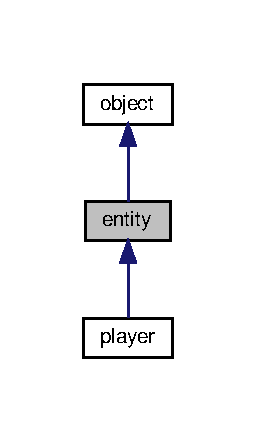
\includegraphics[width=123pt]{classentity__inherit__graph}
\end{center}
\end{figure}


Collaboration diagram for entity\+:
\nopagebreak
\begin{figure}[H]
\begin{center}
\leavevmode
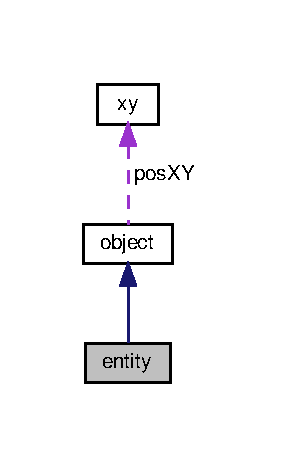
\includegraphics[width=135pt]{classentity__coll__graph}
\end{center}
\end{figure}
\subsection*{Public Member Functions}
\begin{DoxyCompactItemize}
\item 
\hyperlink{classentity_aee3c44b079e4b0909636151b8394fd5b}{entity} (const int \&start\+\_\+x, const int \&start\+\_\+y, char p\+\_\+icon, const float \&speed\+\_\+x, const float \&speed\+\_\+y, const bool \&gravity, const bool \&bounce, const bool \&solid)
\begin{DoxyCompactList}\small\item\em Constructs a entity. \end{DoxyCompactList}\item 
\mbox{\Hypertarget{classentity_ae4d78c5416cd69fbb391cda12a350bfa}\label{classentity_ae4d78c5416cd69fbb391cda12a350bfa}} 
bool {\bfseries get\+\_\+stand} ()
\item 
\mbox{\Hypertarget{classentity_a60593dd7d74e30a73422acd3fc4c7d30}\label{classentity_a60593dd7d74e30a73422acd3fc4c7d30}} 
void {\bfseries set\+\_\+stand} (bool new\+\_\+stand)
\item 
bool \hyperlink{classentity_a3831f4f3b9a07d9fa412909ba2e8d2e7}{get\+\_\+solid} ()
\begin{DoxyCompactList}\small\item\em returns solid \end{DoxyCompactList}\item 
char \hyperlink{classentity_a7be4922bae8e57cb46947b752d6ee5b7}{get\+\_\+icon} ()
\begin{DoxyCompactList}\small\item\em returns icon \end{DoxyCompactList}\item 
float \hyperlink{classentity_a13d173e3d5dd4b669fc88180644b6ae4}{get\+\_\+speed\+\_\+x} ()
\begin{DoxyCompactList}\small\item\em returns x speed \end{DoxyCompactList}\item 
void \hyperlink{classentity_ab07ddec04048c0711a3684d49ae8fa91}{set\+\_\+speed\+\_\+x} (float new\+\_\+speed)
\begin{DoxyCompactList}\small\item\em sets x speed \end{DoxyCompactList}\item 
float \hyperlink{classentity_aac6ef6881c0a334a6cca1c321ffd6066}{get\+\_\+speed\+\_\+y} ()
\begin{DoxyCompactList}\small\item\em returns yspeed \end{DoxyCompactList}\item 
void \hyperlink{classentity_a64a214c123d3ede336ea6989c05063e7}{set\+\_\+speed\+\_\+y} (float new\+\_\+speed)
\begin{DoxyCompactList}\small\item\em sets y speed \end{DoxyCompactList}\item 
bool \hyperlink{classentity_a2e69aae60dda8b7a1b381f7e99f6913f}{get\+\_\+gravity} ()
\begin{DoxyCompactList}\small\item\em returns gravity \end{DoxyCompactList}\item 
bool \hyperlink{classentity_a0c3bddcd6f6512eb0826dfebc90e5b05}{get\+\_\+bounce} ()
\begin{DoxyCompactList}\small\item\em returns bounce \end{DoxyCompactList}\end{DoxyCompactItemize}
\subsection*{Public Attributes}
\begin{DoxyCompactItemize}
\item 
\mbox{\Hypertarget{classentity_ae208c1d4002534e9c82d9c27c4b6d121}\label{classentity_ae208c1d4002534e9c82d9c27c4b6d121}} 
unsigned int {\bfseries score} = 0
\end{DoxyCompactItemize}
\subsection*{Protected Attributes}
\begin{DoxyCompactItemize}
\item 
\mbox{\Hypertarget{classentity_a276f34d880f0f31f9cd057e6568af672}\label{classentity_a276f34d880f0f31f9cd057e6568af672}} 
char {\bfseries icon}
\item 
\mbox{\Hypertarget{classentity_ade26db2645e09e5cc93dea7688d158bb}\label{classentity_ade26db2645e09e5cc93dea7688d158bb}} 
float {\bfseries speed\+\_\+x}
\item 
\mbox{\Hypertarget{classentity_acfd9a2ea16306a4728fdc712b55732c0}\label{classentity_acfd9a2ea16306a4728fdc712b55732c0}} 
float {\bfseries speed\+\_\+y}
\item 
\mbox{\Hypertarget{classentity_a66debba3d886c74a8f7b39a4f173d02e}\label{classentity_a66debba3d886c74a8f7b39a4f173d02e}} 
bool {\bfseries gravity}
\item 
\mbox{\Hypertarget{classentity_aa2f2b1ebf9dccdf263ae7559b8ddf0bc}\label{classentity_aa2f2b1ebf9dccdf263ae7559b8ddf0bc}} 
bool {\bfseries bounce}
\item 
\mbox{\Hypertarget{classentity_a1284d3366a58d5a6655bb7899e323533}\label{classentity_a1284d3366a58d5a6655bb7899e323533}} 
bool {\bfseries stand} = 0
\item 
\mbox{\Hypertarget{classentity_a743f264f8bcb5ac53e4e28ab88ace871}\label{classentity_a743f264f8bcb5ac53e4e28ab88ace871}} 
int {\bfseries health} = 100
\item 
\mbox{\Hypertarget{classentity_a1aeb8437d4a5a56ef92dad3589ce0f88}\label{classentity_a1aeb8437d4a5a56ef92dad3589ce0f88}} 
float {\bfseries strength} = 1
\item 
\mbox{\Hypertarget{classentity_a7d0545e294792e49ad9e48f56f1863c2}\label{classentity_a7d0545e294792e49ad9e48f56f1863c2}} 
float {\bfseries weight} = 1
\item 
\mbox{\Hypertarget{classentity_a0d9dca7195de473ad176923db9a7e073}\label{classentity_a0d9dca7195de473ad176923db9a7e073}} 
bool {\bfseries solid}
\end{DoxyCompactItemize}


\subsection{Detailed Description}
A visable entity. 

An entity that has an icon, a speed and optionally gravity and other physics. 

\subsection{Constructor \& Destructor Documentation}
\mbox{\Hypertarget{classentity_aee3c44b079e4b0909636151b8394fd5b}\label{classentity_aee3c44b079e4b0909636151b8394fd5b}} 
\index{entity@{entity}!entity@{entity}}
\index{entity@{entity}!entity@{entity}}
\subsubsection{\texorpdfstring{entity()}{entity()}}
{\footnotesize\ttfamily entity\+::entity (\begin{DoxyParamCaption}\item[{const int \&}]{start\+\_\+x,  }\item[{const int \&}]{start\+\_\+y,  }\item[{char}]{p\+\_\+icon,  }\item[{const float \&}]{speed\+\_\+x,  }\item[{const float \&}]{speed\+\_\+y,  }\item[{const bool \&}]{gravity,  }\item[{const bool \&}]{bounce,  }\item[{const bool \&}]{solid }\end{DoxyParamCaption})\hspace{0.3cm}{\ttfamily [inline]}}



Constructs a entity. 

This constructor construct an entity 

\subsection{Member Function Documentation}
\mbox{\Hypertarget{classentity_a0c3bddcd6f6512eb0826dfebc90e5b05}\label{classentity_a0c3bddcd6f6512eb0826dfebc90e5b05}} 
\index{entity@{entity}!get\+\_\+bounce@{get\+\_\+bounce}}
\index{get\+\_\+bounce@{get\+\_\+bounce}!entity@{entity}}
\subsubsection{\texorpdfstring{get\+\_\+bounce()}{get\_bounce()}}
{\footnotesize\ttfamily bool entity\+::get\+\_\+bounce (\begin{DoxyParamCaption}{ }\end{DoxyParamCaption})\hspace{0.3cm}{\ttfamily [inline]}}



returns bounce 

This function returns if the object can bounce \mbox{\Hypertarget{classentity_a2e69aae60dda8b7a1b381f7e99f6913f}\label{classentity_a2e69aae60dda8b7a1b381f7e99f6913f}} 
\index{entity@{entity}!get\+\_\+gravity@{get\+\_\+gravity}}
\index{get\+\_\+gravity@{get\+\_\+gravity}!entity@{entity}}
\subsubsection{\texorpdfstring{get\+\_\+gravity()}{get\_gravity()}}
{\footnotesize\ttfamily bool entity\+::get\+\_\+gravity (\begin{DoxyParamCaption}{ }\end{DoxyParamCaption})\hspace{0.3cm}{\ttfamily [inline]}}



returns gravity 

This function returns if this entity can be affected by gravity. \mbox{\Hypertarget{classentity_a7be4922bae8e57cb46947b752d6ee5b7}\label{classentity_a7be4922bae8e57cb46947b752d6ee5b7}} 
\index{entity@{entity}!get\+\_\+icon@{get\+\_\+icon}}
\index{get\+\_\+icon@{get\+\_\+icon}!entity@{entity}}
\subsubsection{\texorpdfstring{get\+\_\+icon()}{get\_icon()}}
{\footnotesize\ttfamily char entity\+::get\+\_\+icon (\begin{DoxyParamCaption}{ }\end{DoxyParamCaption})\hspace{0.3cm}{\ttfamily [inline]}}



returns icon 

This function returns entity\textquotesingle{}s icon. \mbox{\Hypertarget{classentity_a3831f4f3b9a07d9fa412909ba2e8d2e7}\label{classentity_a3831f4f3b9a07d9fa412909ba2e8d2e7}} 
\index{entity@{entity}!get\+\_\+solid@{get\+\_\+solid}}
\index{get\+\_\+solid@{get\+\_\+solid}!entity@{entity}}
\subsubsection{\texorpdfstring{get\+\_\+solid()}{get\_solid()}}
{\footnotesize\ttfamily bool entity\+::get\+\_\+solid (\begin{DoxyParamCaption}{ }\end{DoxyParamCaption})\hspace{0.3cm}{\ttfamily [inline]}}



returns solid 

returns if the object is solid \mbox{\Hypertarget{classentity_a13d173e3d5dd4b669fc88180644b6ae4}\label{classentity_a13d173e3d5dd4b669fc88180644b6ae4}} 
\index{entity@{entity}!get\+\_\+speed\+\_\+x@{get\+\_\+speed\+\_\+x}}
\index{get\+\_\+speed\+\_\+x@{get\+\_\+speed\+\_\+x}!entity@{entity}}
\subsubsection{\texorpdfstring{get\+\_\+speed\+\_\+x()}{get\_speed\_x()}}
{\footnotesize\ttfamily float entity\+::get\+\_\+speed\+\_\+x (\begin{DoxyParamCaption}{ }\end{DoxyParamCaption})\hspace{0.3cm}{\ttfamily [inline]}}



returns x speed 

This function returns the x speed of object. \mbox{\Hypertarget{classentity_aac6ef6881c0a334a6cca1c321ffd6066}\label{classentity_aac6ef6881c0a334a6cca1c321ffd6066}} 
\index{entity@{entity}!get\+\_\+speed\+\_\+y@{get\+\_\+speed\+\_\+y}}
\index{get\+\_\+speed\+\_\+y@{get\+\_\+speed\+\_\+y}!entity@{entity}}
\subsubsection{\texorpdfstring{get\+\_\+speed\+\_\+y()}{get\_speed\_y()}}
{\footnotesize\ttfamily float entity\+::get\+\_\+speed\+\_\+y (\begin{DoxyParamCaption}{ }\end{DoxyParamCaption})\hspace{0.3cm}{\ttfamily [inline]}}



returns yspeed 

returns entity\textquotesingle{}s float variabel named speed\+\_\+y. \mbox{\Hypertarget{classentity_ab07ddec04048c0711a3684d49ae8fa91}\label{classentity_ab07ddec04048c0711a3684d49ae8fa91}} 
\index{entity@{entity}!set\+\_\+speed\+\_\+x@{set\+\_\+speed\+\_\+x}}
\index{set\+\_\+speed\+\_\+x@{set\+\_\+speed\+\_\+x}!entity@{entity}}
\subsubsection{\texorpdfstring{set\+\_\+speed\+\_\+x()}{set\_speed\_x()}}
{\footnotesize\ttfamily void entity\+::set\+\_\+speed\+\_\+x (\begin{DoxyParamCaption}\item[{float}]{new\+\_\+speed }\end{DoxyParamCaption})\hspace{0.3cm}{\ttfamily [inline]}}



sets x speed 

This function sets entity\textquotesingle{}s x speed to given speed. \mbox{\Hypertarget{classentity_a64a214c123d3ede336ea6989c05063e7}\label{classentity_a64a214c123d3ede336ea6989c05063e7}} 
\index{entity@{entity}!set\+\_\+speed\+\_\+y@{set\+\_\+speed\+\_\+y}}
\index{set\+\_\+speed\+\_\+y@{set\+\_\+speed\+\_\+y}!entity@{entity}}
\subsubsection{\texorpdfstring{set\+\_\+speed\+\_\+y()}{set\_speed\_y()}}
{\footnotesize\ttfamily void entity\+::set\+\_\+speed\+\_\+y (\begin{DoxyParamCaption}\item[{float}]{new\+\_\+speed }\end{DoxyParamCaption})\hspace{0.3cm}{\ttfamily [inline]}}



sets y speed 

This function sets entity\textquotesingle{}s y speed to given speed. 

The documentation for this class was generated from the following file\+:\begin{DoxyCompactItemize}
\item 
src/\+Matrix\+Engine/\hyperlink{object_8h}{object.\+h}\end{DoxyCompactItemize}

\hypertarget{classfield}{}\section{field Class Reference}
\label{classfield}\index{field@{field}}


Entire playground of the scene.  




{\ttfamily \#include $<$field.\+h$>$}

\subsection*{Public Member Functions}
\begin{DoxyCompactItemize}
\item 
\hyperlink{classfield_aed35371ff99892965f46835a32b57c41}{field} (const int \&x\+\_\+size, const int \&y\+\_\+size)
\begin{DoxyCompactList}\small\item\em Constructor of field class. \end{DoxyCompactList}\item 
int \hyperlink{classfield_a87f95797eadbc2b60276d4503383bef0}{get\+\_\+x} ()
\begin{DoxyCompactList}\small\item\em Returns x. \end{DoxyCompactList}\item 
int \hyperlink{classfield_aa5aad6f7a49d4265ec8c482030553a18}{get\+\_\+y} ()
\begin{DoxyCompactList}\small\item\em Returns y. \end{DoxyCompactList}\item 
void \hyperlink{classfield_acebf59882faff84102c239ac6ab63a09}{create} ()
\begin{DoxyCompactList}\small\item\em Initialises all the empty spaces in the Playground Array. \end{DoxyCompactList}\item 
void \hyperlink{classfield_a25b067a824200a97e2795a063b440684}{draw} (\hyperlink{classentity}{entity} \&obj)
\begin{DoxyCompactList}\small\item\em Writes character to 2d Array. \end{DoxyCompactList}\item 
void \hyperlink{classfield_aa52bcbf98c07608197780e1e6cdfaab5}{draw} (\hyperlink{classobstacle}{obstacle} \&obst)
\begin{DoxyCompactList}\small\item\em Writes character to 2d Array. \end{DoxyCompactList}\item 
void \hyperlink{classfield_a5a46a87df8d359135e5dabd900a92546}{clear\+\_\+buffer} ()
\begin{DoxyCompactList}\small\item\em Clears screen buffer. \end{DoxyCompactList}\item 
\hyperlink{classposTouch}{pos\+Touch} \hyperlink{classfield_a272e79e7579f8485f9d082629fd23eae}{get\+\_\+touch} (\hyperlink{classentity}{entity} \&obj)
\begin{DoxyCompactList}\small\item\em Returns \hyperlink{classposTouch}{pos\+Touch} of entity in the Playground Array. \end{DoxyCompactList}\item 
\mbox{\Hypertarget{classfield_a27393334b27b02ba0d6ce08c7104291f}\label{classfield_a27393334b27b02ba0d6ce08c7104291f}} 
void {\bfseries get} (char new\+\_\+scene\mbox{[}Y\+\_\+\+S\+I\+ZE\mbox{]}\mbox{[}X\+\_\+\+S\+I\+ZE\mbox{]})
\item 
\mbox{\Hypertarget{classfield_a529a3a3c6fe009ffdf5356973b3cca13}\label{classfield_a529a3a3c6fe009ffdf5356973b3cca13}} 
void {\bfseries set} (char new\+\_\+scene\mbox{[}Y\+\_\+\+S\+I\+ZE\mbox{]}\mbox{[}X\+\_\+\+S\+I\+ZE\mbox{]})
\end{DoxyCompactItemize}
\subsection*{Public Attributes}
\begin{DoxyCompactItemize}
\item 
\mbox{\Hypertarget{classfield_a26c28b0180722e9a76dd3ee8b3ef3c95}\label{classfield_a26c28b0180722e9a76dd3ee8b3ef3c95}} 
char {\bfseries playground} \mbox{[}Y\+\_\+\+S\+I\+ZE\mbox{]}\mbox{[}X\+\_\+\+S\+I\+ZE\mbox{]} = \{\{\textquotesingle{}.\textquotesingle{}\}\}
\end{DoxyCompactItemize}


\subsection{Detailed Description}
Entire playground of the scene. 

A class that contains a 2d array of characters with a x and an y size. 

\subsection{Constructor \& Destructor Documentation}
\mbox{\Hypertarget{classfield_aed35371ff99892965f46835a32b57c41}\label{classfield_aed35371ff99892965f46835a32b57c41}} 
\index{field@{field}!field@{field}}
\index{field@{field}!field@{field}}
\subsubsection{\texorpdfstring{field()}{field()}}
{\footnotesize\ttfamily field\+::field (\begin{DoxyParamCaption}\item[{const int \&}]{x\+\_\+size,  }\item[{const int \&}]{y\+\_\+size }\end{DoxyParamCaption})\hspace{0.3cm}{\ttfamily [inline]}}



Constructor of field class. 

Constructor of field class, takes in a x size and y size and initialises a 2d array with those sizes. 

\subsection{Member Function Documentation}
\mbox{\Hypertarget{classfield_a5a46a87df8d359135e5dabd900a92546}\label{classfield_a5a46a87df8d359135e5dabd900a92546}} 
\index{field@{field}!clear\+\_\+buffer@{clear\+\_\+buffer}}
\index{clear\+\_\+buffer@{clear\+\_\+buffer}!field@{field}}
\subsubsection{\texorpdfstring{clear\+\_\+buffer()}{clear\_buffer()}}
{\footnotesize\ttfamily void field\+::clear\+\_\+buffer (\begin{DoxyParamCaption}{ }\end{DoxyParamCaption})\hspace{0.3cm}{\ttfamily [inline]}}



Clears screen buffer. 

This function clears the Playground array buffer. \mbox{\Hypertarget{classfield_acebf59882faff84102c239ac6ab63a09}\label{classfield_acebf59882faff84102c239ac6ab63a09}} 
\index{field@{field}!create@{create}}
\index{create@{create}!field@{field}}
\subsubsection{\texorpdfstring{create()}{create()}}
{\footnotesize\ttfamily void field\+::create (\begin{DoxyParamCaption}{ }\end{DoxyParamCaption})}



Initialises all the empty spaces in the Playground Array. 

function initialises all the empty spaces in the Playground Array. \mbox{\Hypertarget{classfield_a25b067a824200a97e2795a063b440684}\label{classfield_a25b067a824200a97e2795a063b440684}} 
\index{field@{field}!draw@{draw}}
\index{draw@{draw}!field@{field}}
\subsubsection{\texorpdfstring{draw()}{draw()}\hspace{0.1cm}{\footnotesize\ttfamily [1/2]}}
{\footnotesize\ttfamily void field\+::draw (\begin{DoxyParamCaption}\item[{\hyperlink{classentity}{entity} \&}]{obj }\end{DoxyParamCaption})}



Writes character to 2d Array. 

This function writes a givin character to the Playground Array. \mbox{\Hypertarget{classfield_aa52bcbf98c07608197780e1e6cdfaab5}\label{classfield_aa52bcbf98c07608197780e1e6cdfaab5}} 
\index{field@{field}!draw@{draw}}
\index{draw@{draw}!field@{field}}
\subsubsection{\texorpdfstring{draw()}{draw()}\hspace{0.1cm}{\footnotesize\ttfamily [2/2]}}
{\footnotesize\ttfamily void field\+::draw (\begin{DoxyParamCaption}\item[{\hyperlink{classobstacle}{obstacle} \&}]{obst }\end{DoxyParamCaption})}



Writes character to 2d Array. 

This function writes a givin character to the Playground Array. \mbox{\Hypertarget{classfield_a272e79e7579f8485f9d082629fd23eae}\label{classfield_a272e79e7579f8485f9d082629fd23eae}} 
\index{field@{field}!get\+\_\+touch@{get\+\_\+touch}}
\index{get\+\_\+touch@{get\+\_\+touch}!field@{field}}
\subsubsection{\texorpdfstring{get\+\_\+touch()}{get\_touch()}}
{\footnotesize\ttfamily \hyperlink{classposTouch}{pos\+Touch} field\+::get\+\_\+touch (\begin{DoxyParamCaption}\item[{\hyperlink{classentity}{entity} \&}]{obj }\end{DoxyParamCaption})}



Returns \hyperlink{classposTouch}{pos\+Touch} of entity in the Playground Array. 

This function returns \hyperlink{classposTouch}{pos\+Touch} of a givin entity in the the Playground Array. \mbox{\Hypertarget{classfield_a87f95797eadbc2b60276d4503383bef0}\label{classfield_a87f95797eadbc2b60276d4503383bef0}} 
\index{field@{field}!get\+\_\+x@{get\+\_\+x}}
\index{get\+\_\+x@{get\+\_\+x}!field@{field}}
\subsubsection{\texorpdfstring{get\+\_\+x()}{get\_x()}}
{\footnotesize\ttfamily int field\+::get\+\_\+x (\begin{DoxyParamCaption}{ }\end{DoxyParamCaption})\hspace{0.3cm}{\ttfamily [inline]}}



Returns x. 

This function returns x \mbox{\Hypertarget{classfield_aa5aad6f7a49d4265ec8c482030553a18}\label{classfield_aa5aad6f7a49d4265ec8c482030553a18}} 
\index{field@{field}!get\+\_\+y@{get\+\_\+y}}
\index{get\+\_\+y@{get\+\_\+y}!field@{field}}
\subsubsection{\texorpdfstring{get\+\_\+y()}{get\_y()}}
{\footnotesize\ttfamily int field\+::get\+\_\+y (\begin{DoxyParamCaption}{ }\end{DoxyParamCaption})\hspace{0.3cm}{\ttfamily [inline]}}



Returns y. 

This function returns y 

The documentation for this class was generated from the following files\+:\begin{DoxyCompactItemize}
\item 
src/\+Matrix\+Engine/\hyperlink{field_8h}{field.\+h}\item 
src/\+Matrix\+Engine/field.\+cpp\end{DoxyCompactItemize}

\hypertarget{classled__matrix}{}\section{led\+\_\+matrix Class Reference}
\label{classled__matrix}\index{led\+\_\+matrix@{led\+\_\+matrix}}


Interface for the M\+H7219 led matrix chip.  




{\ttfamily \#include $<$led\+\_\+matrix.\+hpp$>$}



Inheritance diagram for led\+\_\+matrix\+:
\nopagebreak
\begin{figure}[H]
\begin{center}
\leavevmode
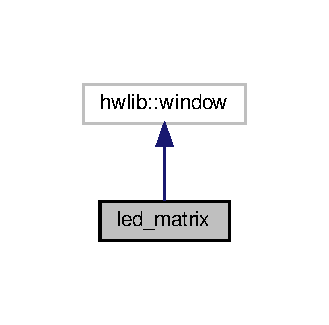
\includegraphics[width=158pt]{classled__matrix__inherit__graph}
\end{center}
\end{figure}


Collaboration diagram for led\+\_\+matrix\+:
\nopagebreak
\begin{figure}[H]
\begin{center}
\leavevmode
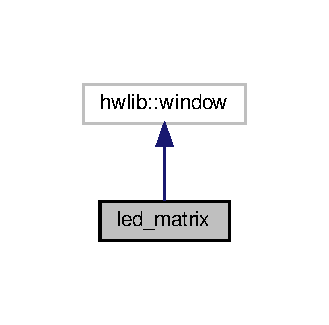
\includegraphics[width=158pt]{classled__matrix__coll__graph}
\end{center}
\end{figure}
\subsection*{Public Member Functions}
\begin{DoxyCompactItemize}
\item 
\hyperlink{classled__matrix_a4b06df3b2766cfde525f14e545d42178}{led\+\_\+matrix} (hwlib\+::spi\+\_\+bus\+\_\+bit\+\_\+banged\+\_\+sclk\+\_\+mosi\+\_\+miso \&spi, hwlib\+::target\+::pin\+\_\+out \&cs)
\begin{DoxyCompactList}\small\item\em Constructor of M\+H7219 interface. \end{DoxyCompactList}\item 
void \hyperlink{classled__matrix_aaaf3d4913c14f5c4f3fda0bab4d2c2d7}{wake} ()
\begin{DoxyCompactList}\small\item\em Wakes up the Led Matrix. \end{DoxyCompactList}\item 
void \hyperlink{classled__matrix_ac926b398f60702bf06e1c6582c04ed6e}{sleep} ()
\begin{DoxyCompactList}\small\item\em Tugs in the Led Matrix. \end{DoxyCompactList}\item 
void \hyperlink{classled__matrix_a074e1d86a05e2e67a3c329d589b601b8}{flush} () override
\begin{DoxyCompactList}\small\item\em the buffer to the Led Matrix. \end{DoxyCompactList}\item 
void \hyperlink{classled__matrix_a0916fce5a976a46da16204265332015f}{flush\+\_\+buffer} (uint8\+\_\+t buffer\mbox{[}8\mbox{]})
\begin{DoxyCompactList}\small\item\em givin buffer to the Led Matrix \end{DoxyCompactList}\item 
void \hyperlink{classled__matrix_af26ac982e5c74a357f5fe18e73b819e4}{clear\+\_\+buffer} ()
\begin{DoxyCompactList}\small\item\em buffer \end{DoxyCompactList}\item 
void \hyperlink{classled__matrix_ac92b3805e1af58f4591bf22402c11d7e}{clear} ()
\begin{DoxyCompactList}\small\item\em Led Matrix Screen \end{DoxyCompactList}\item 
void \hyperlink{classled__matrix_a97602fdecff69971987941e12bc52a0f}{number} (int number)
\begin{DoxyCompactList}\small\item\em a number on Led Matrix \end{DoxyCompactList}\end{DoxyCompactItemize}


\subsection{Detailed Description}
Interface for the M\+H7219 led matrix chip. 

Interface for one M\+H7219 led matrix chip to turn selected pixels on and off using a function. This class is designed to be used with the M\+H7219 Led Matrix 

\subsection{Constructor \& Destructor Documentation}
\mbox{\Hypertarget{classled__matrix_a4b06df3b2766cfde525f14e545d42178}\label{classled__matrix_a4b06df3b2766cfde525f14e545d42178}} 
\index{led\+\_\+matrix@{led\+\_\+matrix}!led\+\_\+matrix@{led\+\_\+matrix}}
\index{led\+\_\+matrix@{led\+\_\+matrix}!led\+\_\+matrix@{led\+\_\+matrix}}
\subsubsection{\texorpdfstring{led\+\_\+matrix()}{led\_matrix()}}
{\footnotesize\ttfamily led\+\_\+matrix\+::led\+\_\+matrix (\begin{DoxyParamCaption}\item[{hwlib\+::spi\+\_\+bus\+\_\+bit\+\_\+banged\+\_\+sclk\+\_\+mosi\+\_\+miso \&}]{spi,  }\item[{hwlib\+::target\+::pin\+\_\+out \&}]{cs }\end{DoxyParamCaption})\hspace{0.3cm}{\ttfamily [inline]}}



Constructor of M\+H7219 interface. 

This is the constructor of the M\+H7219 interface. 

\subsection{Member Function Documentation}
\mbox{\Hypertarget{classled__matrix_ac92b3805e1af58f4591bf22402c11d7e}\label{classled__matrix_ac92b3805e1af58f4591bf22402c11d7e}} 
\index{led\+\_\+matrix@{led\+\_\+matrix}!clear@{clear}}
\index{clear@{clear}!led\+\_\+matrix@{led\+\_\+matrix}}
\subsubsection{\texorpdfstring{clear()}{clear()}}
{\footnotesize\ttfamily void led\+\_\+matrix\+::clear (\begin{DoxyParamCaption}{ }\end{DoxyParamCaption})\hspace{0.3cm}{\ttfamily [inline]}}



Led Matrix Screen 

function clears the current displayed pixels on the Led Matrix \mbox{\Hypertarget{classled__matrix_af26ac982e5c74a357f5fe18e73b819e4}\label{classled__matrix_af26ac982e5c74a357f5fe18e73b819e4}} 
\index{led\+\_\+matrix@{led\+\_\+matrix}!clear\+\_\+buffer@{clear\+\_\+buffer}}
\index{clear\+\_\+buffer@{clear\+\_\+buffer}!led\+\_\+matrix@{led\+\_\+matrix}}
\subsubsection{\texorpdfstring{clear\+\_\+buffer()}{clear\_buffer()}}
{\footnotesize\ttfamily void led\+\_\+matrix\+::clear\+\_\+buffer (\begin{DoxyParamCaption}{ }\end{DoxyParamCaption})\hspace{0.3cm}{\ttfamily [inline]}}



buffer 

function clears the current screen buffer \mbox{\Hypertarget{classled__matrix_a074e1d86a05e2e67a3c329d589b601b8}\label{classled__matrix_a074e1d86a05e2e67a3c329d589b601b8}} 
\index{led\+\_\+matrix@{led\+\_\+matrix}!flush@{flush}}
\index{flush@{flush}!led\+\_\+matrix@{led\+\_\+matrix}}
\subsubsection{\texorpdfstring{flush()}{flush()}}
{\footnotesize\ttfamily void led\+\_\+matrix\+::flush (\begin{DoxyParamCaption}{ }\end{DoxyParamCaption})\hspace{0.3cm}{\ttfamily [inline]}, {\ttfamily [override]}}



the buffer to the Led Matrix. 

function writes the screen buffer array to the Led Matrix \mbox{\Hypertarget{classled__matrix_a0916fce5a976a46da16204265332015f}\label{classled__matrix_a0916fce5a976a46da16204265332015f}} 
\index{led\+\_\+matrix@{led\+\_\+matrix}!flush\+\_\+buffer@{flush\+\_\+buffer}}
\index{flush\+\_\+buffer@{flush\+\_\+buffer}!led\+\_\+matrix@{led\+\_\+matrix}}
\subsubsection{\texorpdfstring{flush\+\_\+buffer()}{flush\_buffer()}}
{\footnotesize\ttfamily void led\+\_\+matrix\+::flush\+\_\+buffer (\begin{DoxyParamCaption}\item[{uint8\+\_\+t}]{buffer\mbox{[}8\mbox{]} }\end{DoxyParamCaption})\hspace{0.3cm}{\ttfamily [inline]}}



givin buffer to the Led Matrix 

function is for writing a givin screen buffer to the Led Matrix \mbox{\Hypertarget{classled__matrix_a97602fdecff69971987941e12bc52a0f}\label{classled__matrix_a97602fdecff69971987941e12bc52a0f}} 
\index{led\+\_\+matrix@{led\+\_\+matrix}!number@{number}}
\index{number@{number}!led\+\_\+matrix@{led\+\_\+matrix}}
\subsubsection{\texorpdfstring{number()}{number()}}
{\footnotesize\ttfamily void led\+\_\+matrix\+::number (\begin{DoxyParamCaption}\item[{int}]{number }\end{DoxyParamCaption})\hspace{0.3cm}{\ttfamily [inline]}}



a number on Led Matrix 

Function displays a givin number on the Led Matrix \mbox{\Hypertarget{classled__matrix_ac926b398f60702bf06e1c6582c04ed6e}\label{classled__matrix_ac926b398f60702bf06e1c6582c04ed6e}} 
\index{led\+\_\+matrix@{led\+\_\+matrix}!sleep@{sleep}}
\index{sleep@{sleep}!led\+\_\+matrix@{led\+\_\+matrix}}
\subsubsection{\texorpdfstring{sleep()}{sleep()}}
{\footnotesize\ttfamily void led\+\_\+matrix\+::sleep (\begin{DoxyParamCaption}{ }\end{DoxyParamCaption})\hspace{0.3cm}{\ttfamily [inline]}}



Tugs in the Led Matrix. 

Sends a sleep bit to the Sleep Register for the M\+H7219 Led Matrix to turn it . \mbox{\Hypertarget{classled__matrix_aaaf3d4913c14f5c4f3fda0bab4d2c2d7}\label{classled__matrix_aaaf3d4913c14f5c4f3fda0bab4d2c2d7}} 
\index{led\+\_\+matrix@{led\+\_\+matrix}!wake@{wake}}
\index{wake@{wake}!led\+\_\+matrix@{led\+\_\+matrix}}
\subsubsection{\texorpdfstring{wake()}{wake()}}
{\footnotesize\ttfamily void led\+\_\+matrix\+::wake (\begin{DoxyParamCaption}{ }\end{DoxyParamCaption})\hspace{0.3cm}{\ttfamily [inline]}}



Wakes up the Led Matrix. 

\textbackslash{} Wakes up the M\+H7219 Led Matrix Chip by sending data to different registers. 

The documentation for this class was generated from the following file\+:\begin{DoxyCompactItemize}
\item 
src/\+Matrix\+Engine/\hyperlink{led__matrix_8hpp}{led\+\_\+matrix.\+hpp}\end{DoxyCompactItemize}

\hypertarget{classobject}{}\section{object Class Reference}
\label{classobject}\index{object@{object}}


A void object with a position.  




{\ttfamily \#include $<$object.\+h$>$}



Inheritance diagram for object\+:
\nopagebreak
\begin{figure}[H]
\begin{center}
\leavevmode
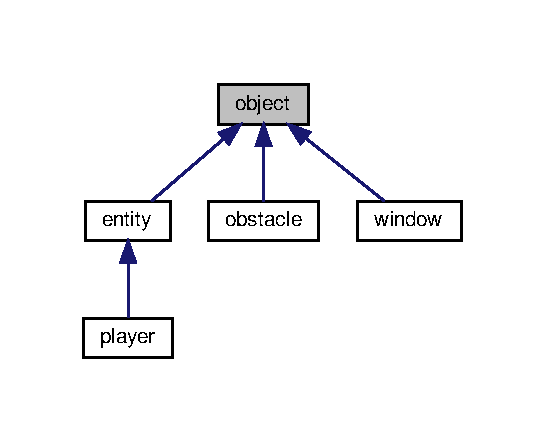
\includegraphics[width=262pt]{classobject__inherit__graph}
\end{center}
\end{figure}


Collaboration diagram for object\+:
\nopagebreak
\begin{figure}[H]
\begin{center}
\leavevmode
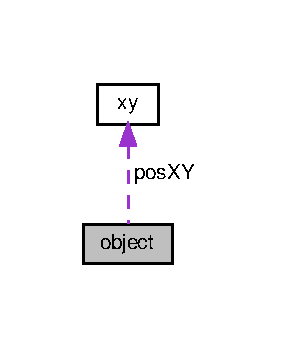
\includegraphics[width=135pt]{classobject__coll__graph}
\end{center}
\end{figure}
\subsection*{Public Member Functions}
\begin{DoxyCompactItemize}
\item 
\mbox{\Hypertarget{classobject_a3266e9f8d8e98fe05314c959f5929c7d}\label{classobject_a3266e9f8d8e98fe05314c959f5929c7d}} 
{\bfseries object} (const int \&start\+\_\+x, const int \&start\+\_\+y)
\item 
virtual int \hyperlink{classobject_a495a093671c8741380a292dd0bc757cb}{get\+\_\+x} ()
\begin{DoxyCompactList}\small\item\em returns x \end{DoxyCompactList}\item 
virtual int \hyperlink{classobject_abc363fe3aa7a4f29b035df6a57695eba}{get\+\_\+y} ()
\begin{DoxyCompactList}\small\item\em returns y \end{DoxyCompactList}\item 
virtual void \hyperlink{classobject_a0520ed913c351f67b3abc458a5896833}{set\+\_\+x} (int u\+\_\+x)
\begin{DoxyCompactList}\small\item\em sets x \end{DoxyCompactList}\item 
virtual void \hyperlink{classobject_af2831ab422aedd6671aa894d78bb5288}{set\+\_\+y} (int u\+\_\+y)
\begin{DoxyCompactList}\small\item\em sets y \end{DoxyCompactList}\item 
void \hyperlink{classobject_a303b713cf517cebb6b56476facc9022f}{set\+\_\+pos} (int x, int y)
\begin{DoxyCompactList}\small\item\em Set position to given coordinates. \end{DoxyCompactList}\item 
void \hyperlink{classobject_afeb4c581ea86494f8063f286664adbe6}{move\+\_\+up} ()
\begin{DoxyCompactList}\small\item\em Subtracts one from x. \end{DoxyCompactList}\item 
void \hyperlink{classobject_a0a8f714e2850552b925383f53c407430}{move\+\_\+down} ()
\begin{DoxyCompactList}\small\item\em Adds Sone from x. \end{DoxyCompactList}\item 
void \hyperlink{classobject_a60b38349b8faad4c9e41f08df2c41428}{move\+\_\+left} ()
\begin{DoxyCompactList}\small\item\em Subtracts one from y. \end{DoxyCompactList}\item 
void \hyperlink{classobject_aeee28bb1b3f967e374c2878ddc4c57df}{move\+\_\+right} ()
\begin{DoxyCompactList}\small\item\em Adds one from y. \end{DoxyCompactList}\end{DoxyCompactItemize}
\subsection*{Protected Attributes}
\begin{DoxyCompactItemize}
\item 
\hyperlink{classxy}{xy} \hyperlink{classobject_a7fc771aa9781b84b7ee9d222c9bfa605}{pos\+XY}
\begin{DoxyCompactList}\small\item\em position of object \end{DoxyCompactList}\end{DoxyCompactItemize}


\subsection{Detailed Description}
A void object with a position. 

A void object with a position, an object on its own is invisable inside a frame because it\textquotesingle{}s a void. 

\subsection{Member Function Documentation}
\mbox{\Hypertarget{classobject_a495a093671c8741380a292dd0bc757cb}\label{classobject_a495a093671c8741380a292dd0bc757cb}} 
\index{object@{object}!get\+\_\+x@{get\+\_\+x}}
\index{get\+\_\+x@{get\+\_\+x}!object@{object}}
\subsubsection{\texorpdfstring{get\+\_\+x()}{get\_x()}}
{\footnotesize\ttfamily virtual int object\+::get\+\_\+x (\begin{DoxyParamCaption}{ }\end{DoxyParamCaption})\hspace{0.3cm}{\ttfamily [inline]}, {\ttfamily [virtual]}}



returns x 

returns x position of the object \mbox{\Hypertarget{classobject_abc363fe3aa7a4f29b035df6a57695eba}\label{classobject_abc363fe3aa7a4f29b035df6a57695eba}} 
\index{object@{object}!get\+\_\+y@{get\+\_\+y}}
\index{get\+\_\+y@{get\+\_\+y}!object@{object}}
\subsubsection{\texorpdfstring{get\+\_\+y()}{get\_y()}}
{\footnotesize\ttfamily virtual int object\+::get\+\_\+y (\begin{DoxyParamCaption}{ }\end{DoxyParamCaption})\hspace{0.3cm}{\ttfamily [inline]}, {\ttfamily [virtual]}}



returns y 

returns y position of the object \mbox{\Hypertarget{classobject_a0a8f714e2850552b925383f53c407430}\label{classobject_a0a8f714e2850552b925383f53c407430}} 
\index{object@{object}!move\+\_\+down@{move\+\_\+down}}
\index{move\+\_\+down@{move\+\_\+down}!object@{object}}
\subsubsection{\texorpdfstring{move\+\_\+down()}{move\_down()}}
{\footnotesize\ttfamily void object\+::move\+\_\+down (\begin{DoxyParamCaption}{ }\end{DoxyParamCaption})}



Adds Sone from x. 

Moves the object down by one unit adding one to the x position \mbox{\Hypertarget{classobject_a60b38349b8faad4c9e41f08df2c41428}\label{classobject_a60b38349b8faad4c9e41f08df2c41428}} 
\index{object@{object}!move\+\_\+left@{move\+\_\+left}}
\index{move\+\_\+left@{move\+\_\+left}!object@{object}}
\subsubsection{\texorpdfstring{move\+\_\+left()}{move\_left()}}
{\footnotesize\ttfamily void object\+::move\+\_\+left (\begin{DoxyParamCaption}{ }\end{DoxyParamCaption})}



Subtracts one from y. 

Moves the object left by one unit subtracting one to the y position \mbox{\Hypertarget{classobject_aeee28bb1b3f967e374c2878ddc4c57df}\label{classobject_aeee28bb1b3f967e374c2878ddc4c57df}} 
\index{object@{object}!move\+\_\+right@{move\+\_\+right}}
\index{move\+\_\+right@{move\+\_\+right}!object@{object}}
\subsubsection{\texorpdfstring{move\+\_\+right()}{move\_right()}}
{\footnotesize\ttfamily void object\+::move\+\_\+right (\begin{DoxyParamCaption}{ }\end{DoxyParamCaption})}



Adds one from y. 

Moves the object right by one unit by adding one to the y position \mbox{\Hypertarget{classobject_afeb4c581ea86494f8063f286664adbe6}\label{classobject_afeb4c581ea86494f8063f286664adbe6}} 
\index{object@{object}!move\+\_\+up@{move\+\_\+up}}
\index{move\+\_\+up@{move\+\_\+up}!object@{object}}
\subsubsection{\texorpdfstring{move\+\_\+up()}{move\_up()}}
{\footnotesize\ttfamily void object\+::move\+\_\+up (\begin{DoxyParamCaption}{ }\end{DoxyParamCaption})}



Subtracts one from x. 

Moves the object up by one unit subtracting one to the x position \mbox{\Hypertarget{classobject_a303b713cf517cebb6b56476facc9022f}\label{classobject_a303b713cf517cebb6b56476facc9022f}} 
\index{object@{object}!set\+\_\+pos@{set\+\_\+pos}}
\index{set\+\_\+pos@{set\+\_\+pos}!object@{object}}
\subsubsection{\texorpdfstring{set\+\_\+pos()}{set\_pos()}}
{\footnotesize\ttfamily void object\+::set\+\_\+pos (\begin{DoxyParamCaption}\item[{int}]{x,  }\item[{int}]{y }\end{DoxyParamCaption})\hspace{0.3cm}{\ttfamily [inline]}}



Set position to given coordinates. 

This function sets the position of the object to the given x, y coordinates \mbox{\Hypertarget{classobject_a0520ed913c351f67b3abc458a5896833}\label{classobject_a0520ed913c351f67b3abc458a5896833}} 
\index{object@{object}!set\+\_\+x@{set\+\_\+x}}
\index{set\+\_\+x@{set\+\_\+x}!object@{object}}
\subsubsection{\texorpdfstring{set\+\_\+x()}{set\_x()}}
{\footnotesize\ttfamily virtual void object\+::set\+\_\+x (\begin{DoxyParamCaption}\item[{int}]{u\+\_\+x }\end{DoxyParamCaption})\hspace{0.3cm}{\ttfamily [inline]}, {\ttfamily [virtual]}}



sets x 

sets x position of the object \mbox{\Hypertarget{classobject_af2831ab422aedd6671aa894d78bb5288}\label{classobject_af2831ab422aedd6671aa894d78bb5288}} 
\index{object@{object}!set\+\_\+y@{set\+\_\+y}}
\index{set\+\_\+y@{set\+\_\+y}!object@{object}}
\subsubsection{\texorpdfstring{set\+\_\+y()}{set\_y()}}
{\footnotesize\ttfamily virtual void object\+::set\+\_\+y (\begin{DoxyParamCaption}\item[{int}]{u\+\_\+y }\end{DoxyParamCaption})\hspace{0.3cm}{\ttfamily [inline]}, {\ttfamily [virtual]}}



sets y 

sets y position of the objects 

\subsection{Member Data Documentation}
\mbox{\Hypertarget{classobject_a7fc771aa9781b84b7ee9d222c9bfa605}\label{classobject_a7fc771aa9781b84b7ee9d222c9bfa605}} 
\index{object@{object}!pos\+XY@{pos\+XY}}
\index{pos\+XY@{pos\+XY}!object@{object}}
\subsubsection{\texorpdfstring{pos\+XY}{posXY}}
{\footnotesize\ttfamily \hyperlink{classxy}{xy} object\+::pos\+XY\hspace{0.3cm}{\ttfamily [protected]}}



position of object 

x and y position of an object 

The documentation for this class was generated from the following files\+:\begin{DoxyCompactItemize}
\item 
src/\+Matrix\+Engine/\hyperlink{object_8h}{object.\+h}\item 
src/\+Matrix\+Engine/object.\+cpp\end{DoxyCompactItemize}

\hypertarget{classobstacle}{}\section{obstacle Class Reference}
\label{classobstacle}\index{obstacle@{obstacle}}


Solid Object with a start end point.  




{\ttfamily \#include $<$object.\+h$>$}



Inheritance diagram for obstacle\+:
\nopagebreak
\begin{figure}[H]
\begin{center}
\leavevmode
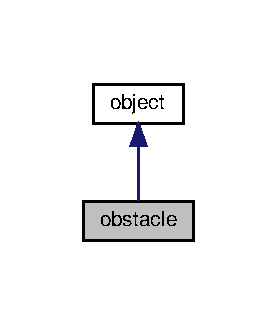
\includegraphics[width=133pt]{classobstacle__inherit__graph}
\end{center}
\end{figure}


Collaboration diagram for obstacle\+:
\nopagebreak
\begin{figure}[H]
\begin{center}
\leavevmode
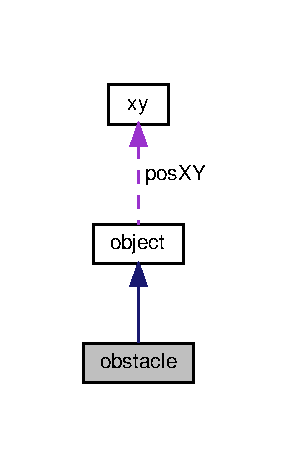
\includegraphics[width=140pt]{classobstacle__coll__graph}
\end{center}
\end{figure}
\subsection*{Public Member Functions}
\begin{DoxyCompactItemize}
\item 
\hyperlink{classobstacle_ac5d3684c209786d12571f8ad09445ffc}{obstacle} (int start\+\_\+x, int start\+\_\+y)
\begin{DoxyCompactList}\small\item\em Constructor of obstacle with only 1 position. \end{DoxyCompactList}\item 
\hyperlink{classobstacle_af3e8b2149760b57bb9238f03bd1616b7}{obstacle} (int start\+\_\+x, int start\+\_\+y, bool passable)
\begin{DoxyCompactList}\small\item\em Constructor of obstacle with only 1 position and if it\textquotesingle{}s solid. \end{DoxyCompactList}\item 
\hyperlink{classobstacle_a39b2e95776adad7254a2fbe0239364a0}{obstacle} (int start\+\_\+x, int start\+\_\+y, int end\+\_\+x, int end\+\_\+y)
\begin{DoxyCompactList}\small\item\em Constructor of obstacle with 2 positions. \end{DoxyCompactList}\item 
\hyperlink{classobstacle_a94dfef60582ffd9f6b08012d61bc4ad3}{obstacle} (int start\+\_\+x, int start\+\_\+y, int end\+\_\+x, int end\+\_\+y, bool passable)
\begin{DoxyCompactList}\small\item\em Constructor of obstacle with 2 positions and if it\textquotesingle{}s solid. \end{DoxyCompactList}\item 
void \hyperlink{classobstacle_af6a9bc32f4999fd9109eda04febdae40}{set\+\_\+pos} (int p\+\_\+start\+\_\+x, int p\+\_\+start\+\_\+y, int p\+\_\+end\+\_\+x, int p\+\_\+end\+\_\+y)
\begin{DoxyCompactList}\small\item\em sets position of obstacle \end{DoxyCompactList}\item 
\mbox{\Hypertarget{classobstacle_a497febf8720e8db38f0d4b385feb192d}\label{classobstacle_a497febf8720e8db38f0d4b385feb192d}} 
int \hyperlink{classobstacle_a497febf8720e8db38f0d4b385feb192d}{get\+\_\+start\+\_\+x} ()
\begin{DoxyCompactList}\small\item\em Returns start x details This function returns the start x value. \end{DoxyCompactList}\item 
\mbox{\Hypertarget{classobstacle_a0166e8c89c16c6c40f87fdae232d160b}\label{classobstacle_a0166e8c89c16c6c40f87fdae232d160b}} 
int \hyperlink{classobstacle_a0166e8c89c16c6c40f87fdae232d160b}{get\+\_\+start\+\_\+y} ()
\begin{DoxyCompactList}\small\item\em Returns start x details This function returns the start x value. \end{DoxyCompactList}\item 
\mbox{\Hypertarget{classobstacle_af51bb5ce1a36f954b39c667a82464046}\label{classobstacle_af51bb5ce1a36f954b39c667a82464046}} 
int \hyperlink{classobstacle_af51bb5ce1a36f954b39c667a82464046}{get\+\_\+end\+\_\+x} ()
\begin{DoxyCompactList}\small\item\em Returns end x details This function returns the end x value. \end{DoxyCompactList}\item 
\mbox{\Hypertarget{classobstacle_add9b03205e5ea6768d70357e9d3f7e08}\label{classobstacle_add9b03205e5ea6768d70357e9d3f7e08}} 
int \hyperlink{classobstacle_add9b03205e5ea6768d70357e9d3f7e08}{get\+\_\+end\+\_\+y} ()
\begin{DoxyCompactList}\small\item\em Returns end x details This function returns the end x value. \end{DoxyCompactList}\item 
\mbox{\Hypertarget{classobstacle_a7eb291920f0286d4bb98b1b6a1e10bf2}\label{classobstacle_a7eb291920f0286d4bb98b1b6a1e10bf2}} 
char \hyperlink{classobstacle_a7eb291920f0286d4bb98b1b6a1e10bf2}{get\+\_\+icon} ()
\begin{DoxyCompactList}\small\item\em Returns icon details This function returns the icon. \end{DoxyCompactList}\end{DoxyCompactItemize}
\subsection*{Additional Inherited Members}


\subsection{Detailed Description}
Solid Object with a start end point. 

This class of an solid object with a start and end position. Normal entities cannot move through an obstacle. 

\subsection{Constructor \& Destructor Documentation}
\mbox{\Hypertarget{classobstacle_ac5d3684c209786d12571f8ad09445ffc}\label{classobstacle_ac5d3684c209786d12571f8ad09445ffc}} 
\index{obstacle@{obstacle}!obstacle@{obstacle}}
\index{obstacle@{obstacle}!obstacle@{obstacle}}
\subsubsection{\texorpdfstring{obstacle()}{obstacle()}\hspace{0.1cm}{\footnotesize\ttfamily [1/4]}}
{\footnotesize\ttfamily obstacle\+::obstacle (\begin{DoxyParamCaption}\item[{int}]{start\+\_\+x,  }\item[{int}]{start\+\_\+y }\end{DoxyParamCaption})\hspace{0.3cm}{\ttfamily [inline]}}



Constructor of obstacle with only 1 position. 

This constructor constructs obstacle with only 1 position \mbox{\Hypertarget{classobstacle_af3e8b2149760b57bb9238f03bd1616b7}\label{classobstacle_af3e8b2149760b57bb9238f03bd1616b7}} 
\index{obstacle@{obstacle}!obstacle@{obstacle}}
\index{obstacle@{obstacle}!obstacle@{obstacle}}
\subsubsection{\texorpdfstring{obstacle()}{obstacle()}\hspace{0.1cm}{\footnotesize\ttfamily [2/4]}}
{\footnotesize\ttfamily obstacle\+::obstacle (\begin{DoxyParamCaption}\item[{int}]{start\+\_\+x,  }\item[{int}]{start\+\_\+y,  }\item[{bool}]{passable }\end{DoxyParamCaption})\hspace{0.3cm}{\ttfamily [inline]}}



Constructor of obstacle with only 1 position and if it\textquotesingle{}s solid. 

This constructor constructs obstacle with only 1 position and if it\textquotesingle{}s solid \mbox{\Hypertarget{classobstacle_a39b2e95776adad7254a2fbe0239364a0}\label{classobstacle_a39b2e95776adad7254a2fbe0239364a0}} 
\index{obstacle@{obstacle}!obstacle@{obstacle}}
\index{obstacle@{obstacle}!obstacle@{obstacle}}
\subsubsection{\texorpdfstring{obstacle()}{obstacle()}\hspace{0.1cm}{\footnotesize\ttfamily [3/4]}}
{\footnotesize\ttfamily obstacle\+::obstacle (\begin{DoxyParamCaption}\item[{int}]{start\+\_\+x,  }\item[{int}]{start\+\_\+y,  }\item[{int}]{end\+\_\+x,  }\item[{int}]{end\+\_\+y }\end{DoxyParamCaption})\hspace{0.3cm}{\ttfamily [inline]}}



Constructor of obstacle with 2 positions. 

This constructor constructs obstacle with 2 positions \mbox{\Hypertarget{classobstacle_a94dfef60582ffd9f6b08012d61bc4ad3}\label{classobstacle_a94dfef60582ffd9f6b08012d61bc4ad3}} 
\index{obstacle@{obstacle}!obstacle@{obstacle}}
\index{obstacle@{obstacle}!obstacle@{obstacle}}
\subsubsection{\texorpdfstring{obstacle()}{obstacle()}\hspace{0.1cm}{\footnotesize\ttfamily [4/4]}}
{\footnotesize\ttfamily obstacle\+::obstacle (\begin{DoxyParamCaption}\item[{int}]{start\+\_\+x,  }\item[{int}]{start\+\_\+y,  }\item[{int}]{end\+\_\+x,  }\item[{int}]{end\+\_\+y,  }\item[{bool}]{passable }\end{DoxyParamCaption})\hspace{0.3cm}{\ttfamily [inline]}}



Constructor of obstacle with 2 positions and if it\textquotesingle{}s solid. 

This constructor constructs obstacle with 2 position and if it\textquotesingle{}s solid 

\subsection{Member Function Documentation}
\mbox{\Hypertarget{classobstacle_af6a9bc32f4999fd9109eda04febdae40}\label{classobstacle_af6a9bc32f4999fd9109eda04febdae40}} 
\index{obstacle@{obstacle}!set\+\_\+pos@{set\+\_\+pos}}
\index{set\+\_\+pos@{set\+\_\+pos}!obstacle@{obstacle}}
\subsubsection{\texorpdfstring{set\+\_\+pos()}{set\_pos()}}
{\footnotesize\ttfamily void obstacle\+::set\+\_\+pos (\begin{DoxyParamCaption}\item[{int}]{p\+\_\+start\+\_\+x,  }\item[{int}]{p\+\_\+start\+\_\+y,  }\item[{int}]{p\+\_\+end\+\_\+x,  }\item[{int}]{p\+\_\+end\+\_\+y }\end{DoxyParamCaption})\hspace{0.3cm}{\ttfamily [inline]}}



sets position of obstacle 

This function sets the 2 postions of an obstacle 

The documentation for this class was generated from the following file\+:\begin{DoxyCompactItemize}
\item 
src/\+Matrix\+Engine/\hyperlink{object_8h}{object.\+h}\end{DoxyCompactItemize}

\hypertarget{classphysbox}{}\section{physbox Class Reference}
\label{classphysbox}\index{physbox@{physbox}}


Physics engine.  




{\ttfamily \#include $<$physics.\+h$>$}

\subsection*{Public Member Functions}
\begin{DoxyCompactItemize}
\item 
void \hyperlink{classphysbox_ab6ae32c018841713b135a1fc511b9518}{calculate\+\_\+movement} (\hyperlink{classentity}{entity} \&\hyperlink{classobject}{object}, \hyperlink{classfield}{field} \&scene)
\begin{DoxyCompactList}\small\item\em Calculates the next movent of entity. \end{DoxyCompactList}\item 
void \hyperlink{classphysbox_aacb7573b68494f352edb2697c5124571}{calculate\+\_\+gravity} (\hyperlink{classentity}{entity} \&\hyperlink{classobject}{object}, \hyperlink{classfield}{field} \&scene)
\begin{DoxyCompactList}\small\item\em Calculates gravity on object. \end{DoxyCompactList}\item 
void \hyperlink{classphysbox_a1e1ca37a18b94e3fab074120e65f7e03}{calculate\+\_\+bounce} (\hyperlink{classentity}{entity} \&\hyperlink{classobject}{object}, \hyperlink{classfield}{field} \&scene)
\begin{DoxyCompactList}\small\item\em Calculates bounce on object. \end{DoxyCompactList}\end{DoxyCompactItemize}


\subsection{Detailed Description}
Physics engine. 

physics engine that calculates basic stuff like gravity speed bouncing and other types of movement 

\subsection{Member Function Documentation}
\mbox{\Hypertarget{classphysbox_a1e1ca37a18b94e3fab074120e65f7e03}\label{classphysbox_a1e1ca37a18b94e3fab074120e65f7e03}} 
\index{physbox@{physbox}!calculate\+\_\+bounce@{calculate\+\_\+bounce}}
\index{calculate\+\_\+bounce@{calculate\+\_\+bounce}!physbox@{physbox}}
\subsubsection{\texorpdfstring{calculate\+\_\+bounce()}{calculate\_bounce()}}
{\footnotesize\ttfamily void physbox\+::calculate\+\_\+bounce (\begin{DoxyParamCaption}\item[{\hyperlink{classentity}{entity} \&}]{object,  }\item[{\hyperlink{classfield}{field} \&}]{scene }\end{DoxyParamCaption})}



Calculates bounce on object. 

This function calculates if the given object should be bouncing in given scene \mbox{\Hypertarget{classphysbox_aacb7573b68494f352edb2697c5124571}\label{classphysbox_aacb7573b68494f352edb2697c5124571}} 
\index{physbox@{physbox}!calculate\+\_\+gravity@{calculate\+\_\+gravity}}
\index{calculate\+\_\+gravity@{calculate\+\_\+gravity}!physbox@{physbox}}
\subsubsection{\texorpdfstring{calculate\+\_\+gravity()}{calculate\_gravity()}}
{\footnotesize\ttfamily void physbox\+::calculate\+\_\+gravity (\begin{DoxyParamCaption}\item[{\hyperlink{classentity}{entity} \&}]{object,  }\item[{\hyperlink{classfield}{field} \&}]{scene }\end{DoxyParamCaption})}



Calculates gravity on object. 

This function calculates the gravity physics of the given object in given scene. \mbox{\Hypertarget{classphysbox_ab6ae32c018841713b135a1fc511b9518}\label{classphysbox_ab6ae32c018841713b135a1fc511b9518}} 
\index{physbox@{physbox}!calculate\+\_\+movement@{calculate\+\_\+movement}}
\index{calculate\+\_\+movement@{calculate\+\_\+movement}!physbox@{physbox}}
\subsubsection{\texorpdfstring{calculate\+\_\+movement()}{calculate\_movement()}}
{\footnotesize\ttfamily void physbox\+::calculate\+\_\+movement (\begin{DoxyParamCaption}\item[{\hyperlink{classentity}{entity} \&}]{object,  }\item[{\hyperlink{classfield}{field} \&}]{scene }\end{DoxyParamCaption})}



Calculates the next movent of entity. 

This function calculates the next movement of the given object in a given scene. 

The documentation for this class was generated from the following files\+:\begin{DoxyCompactItemize}
\item 
src/\+Matrix\+Engine/\hyperlink{physics_8h}{physics.\+h}\item 
src/\+Matrix\+Engine/physics.\+cpp\end{DoxyCompactItemize}

\hypertarget{classplayer}{}\section{player Class Reference}
\label{classplayer}\index{player@{player}}


Inherited class solely made for the frog jump demo.  




{\ttfamily \#include $<$object.\+h$>$}



Inheritance diagram for player\+:
\nopagebreak
\begin{figure}[H]
\begin{center}
\leavevmode
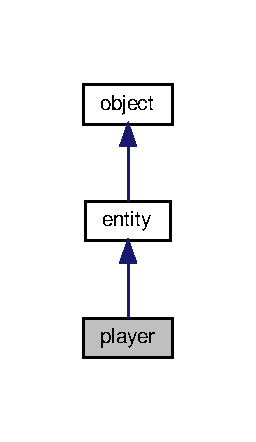
\includegraphics[width=123pt]{classplayer__inherit__graph}
\end{center}
\end{figure}


Collaboration diagram for player\+:
\nopagebreak
\begin{figure}[H]
\begin{center}
\leavevmode
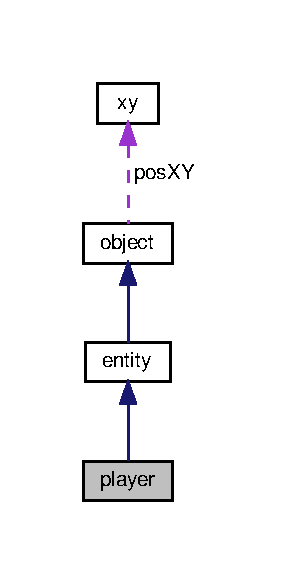
\includegraphics[width=135pt]{classplayer__coll__graph}
\end{center}
\end{figure}
\subsection*{Public Member Functions}
\begin{DoxyCompactItemize}
\item 
\mbox{\Hypertarget{classplayer_a72995ebeb95f9faba238be0217b3eb89}\label{classplayer_a72995ebeb95f9faba238be0217b3eb89}} 
{\bfseries player} (const int \&start\+\_\+x, const int \&start\+\_\+y, char p\+\_\+icon, const float \&speed\+\_\+x, const float \&speed\+\_\+y, const bool \&gravity, const bool \&bounce, const bool \&solid)
\end{DoxyCompactItemize}
\subsection*{Public Attributes}
\begin{DoxyCompactItemize}
\item 
\mbox{\Hypertarget{classplayer_a94bd9c45e32717c2be52f46f4db6755f}\label{classplayer_a94bd9c45e32717c2be52f46f4db6755f}} 
int {\bfseries zone} = 1
\item 
\mbox{\Hypertarget{classplayer_acd04dcecfa678a879e13a26aefa137a2}\label{classplayer_acd04dcecfa678a879e13a26aefa137a2}} 
bool {\bfseries set} = false
\item 
\mbox{\Hypertarget{classplayer_a003957a9fe0e6bef5e23316a44fba858}\label{classplayer_a003957a9fe0e6bef5e23316a44fba858}} 
bool {\bfseries start} = true
\end{DoxyCompactItemize}
\subsection*{Additional Inherited Members}


\subsection{Detailed Description}
Inherited class solely made for the frog jump demo. 

The documentation for this class was generated from the following file\+:\begin{DoxyCompactItemize}
\item 
src/\+Matrix\+Engine/\hyperlink{object_8h}{object.\+h}\end{DoxyCompactItemize}

\hypertarget{classposTouch}{}\section{pos\+Touch Class Reference}
\label{classposTouch}\index{pos\+Touch@{pos\+Touch}}


Collision A\+DT.  




{\ttfamily \#include $<$pos.\+h$>$}

\subsection*{Public Member Functions}
\begin{DoxyCompactItemize}
\item 
\mbox{\Hypertarget{classposTouch_ade8f993b72293c75078b0bffc9d21248}\label{classposTouch_ade8f993b72293c75078b0bffc9d21248}} 
{\bfseries pos\+Touch} (char p\+\_\+up, char p\+\_\+down, char p\+\_\+left, char p\+\_\+right)
\end{DoxyCompactItemize}
\subsection*{Public Attributes}
\begin{DoxyCompactItemize}
\item 
\mbox{\Hypertarget{classposTouch_aef77e026b1e99304109e77e7f57e6ecb}\label{classposTouch_aef77e026b1e99304109e77e7f57e6ecb}} 
char {\bfseries up}
\item 
\mbox{\Hypertarget{classposTouch_a22c07e665a19437432b5119ebcd1e01b}\label{classposTouch_a22c07e665a19437432b5119ebcd1e01b}} 
char {\bfseries down}
\item 
\mbox{\Hypertarget{classposTouch_a395f71bed29f938d2c6d11521853eff1}\label{classposTouch_a395f71bed29f938d2c6d11521853eff1}} 
char {\bfseries left}
\item 
\mbox{\Hypertarget{classposTouch_adab18842bd49d43c45faf4af3b418ac6}\label{classposTouch_adab18842bd49d43c45faf4af3b418ac6}} 
char {\bfseries right}
\end{DoxyCompactItemize}


\subsection{Detailed Description}
Collision A\+DT. 

This class contains the upper character down character left character and right character of a givin object in a field. 

The documentation for this class was generated from the following file\+:\begin{DoxyCompactItemize}
\item 
src/\+Matrix\+Engine/\hyperlink{pos_8h}{pos.\+h}\end{DoxyCompactItemize}

\hypertarget{classwindow}{}\section{window Class Reference}
\label{classwindow}\index{window@{window}}


Renders all data within the sizes and positions.  




{\ttfamily \#include $<$window.\+h$>$}



Inheritance diagram for window\+:
\nopagebreak
\begin{figure}[H]
\begin{center}
\leavevmode
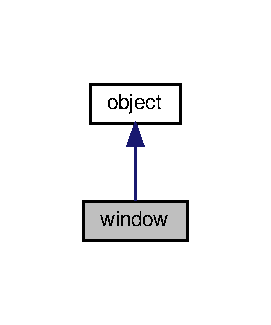
\includegraphics[width=130pt]{classwindow__inherit__graph}
\end{center}
\end{figure}


Collaboration diagram for window\+:
\nopagebreak
\begin{figure}[H]
\begin{center}
\leavevmode
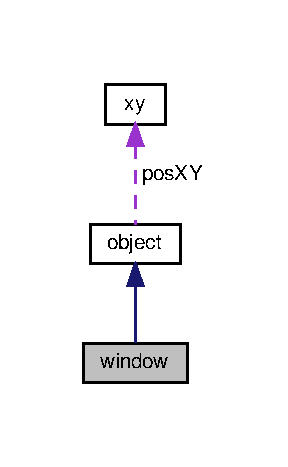
\includegraphics[width=138pt]{classwindow__coll__graph}
\end{center}
\end{figure}
\subsection*{Public Member Functions}
\begin{DoxyCompactItemize}
\item 
\mbox{\Hypertarget{classwindow_a6ea85176a95779f23e6fa96c33dc7dfd}\label{classwindow_a6ea85176a95779f23e6fa96c33dc7dfd}} 
{\bfseries window} (int x, int y, int x\+\_\+size, int y\+\_\+size, \hyperlink{classfield}{field} \&f)
\item 
void \hyperlink{classwindow_aaa5781da14047b439cd587935633ee6d}{draw} ()
\begin{DoxyCompactList}\small\item\em Renders data to terminal. \end{DoxyCompactList}\item 
void \hyperlink{classwindow_a405e7d2c0fcc62a7626c26e82b7a1ae4}{draw} (\hyperlink{classled__matrix}{led\+\_\+matrix} \&display)
\begin{DoxyCompactList}\small\item\em Renders data to 8x8 matrix. \end{DoxyCompactList}\item 
void \hyperlink{classwindow_a398eefc89f338540648fa779de957921}{draw} (hwlib\+::window \&display)
\begin{DoxyCompactList}\small\item\em Renders data to hwlib window. \end{DoxyCompactList}\item 
void \hyperlink{classwindow_aa32da017b225e569e0e3ca6974505873}{move} (\hyperlink{classxy}{xy} start)
\begin{DoxyCompactList}\small\item\em Changes xy pos of frame. \end{DoxyCompactList}\item 
void \hyperlink{classwindow_a6c22ca4ea83cd685762d6c7efb0f228a}{move} (\hyperlink{classxy}{xy} start, \hyperlink{classxy}{xy} end)
\begin{DoxyCompactList}\small\item\em Changes from begin xy to an end xy pos. \end{DoxyCompactList}\item 
void \hyperlink{classwindow_ae668127fa0e1ad8946dcac6a620042b7}{follow} (\hyperlink{classobject}{object} \&obj)
\begin{DoxyCompactList}\small\item\em Frame follows object. \end{DoxyCompactList}\item 
void \hyperlink{classwindow_a83a6b8a998e102def39d0c827d99b48e}{follow\+\_\+y} (\hyperlink{classobject}{object} \&obj)
\begin{DoxyCompactList}\small\item\em Frame follows object. \end{DoxyCompactList}\item 
void \hyperlink{classwindow_a64c6dd5f1f544282541532e17a26d1e7}{follow\+\_\+y} (\hyperlink{classobject}{object} \&obj, int offset)
\begin{DoxyCompactList}\small\item\em Frame follows object. \end{DoxyCompactList}\end{DoxyCompactItemize}
\subsection*{Additional Inherited Members}


\subsection{Detailed Description}
Renders all data within the sizes and positions. 

Window class is similair to a camera in the way that it only renders what it sees. The window class has it\textquotesingle{}s own position inside the field and can follow objects. 

\subsection{Member Function Documentation}
\mbox{\Hypertarget{classwindow_aaa5781da14047b439cd587935633ee6d}\label{classwindow_aaa5781da14047b439cd587935633ee6d}} 
\index{window@{window}!draw@{draw}}
\index{draw@{draw}!window@{window}}
\subsubsection{\texorpdfstring{draw()}{draw()}\hspace{0.1cm}{\footnotesize\ttfamily [1/3]}}
{\footnotesize\ttfamily void window\+::draw (\begin{DoxyParamCaption}{ }\end{DoxyParamCaption})}



Renders data to terminal. 

turns vector data from field into terminal outputs \mbox{\Hypertarget{classwindow_a405e7d2c0fcc62a7626c26e82b7a1ae4}\label{classwindow_a405e7d2c0fcc62a7626c26e82b7a1ae4}} 
\index{window@{window}!draw@{draw}}
\index{draw@{draw}!window@{window}}
\subsubsection{\texorpdfstring{draw()}{draw()}\hspace{0.1cm}{\footnotesize\ttfamily [2/3]}}
{\footnotesize\ttfamily void window\+::draw (\begin{DoxyParamCaption}\item[{\hyperlink{classled__matrix}{led\+\_\+matrix} \&}]{display }\end{DoxyParamCaption})}



Renders data to 8x8 matrix. 

turns array data from field into 8x8 matrix \mbox{\Hypertarget{classwindow_a398eefc89f338540648fa779de957921}\label{classwindow_a398eefc89f338540648fa779de957921}} 
\index{window@{window}!draw@{draw}}
\index{draw@{draw}!window@{window}}
\subsubsection{\texorpdfstring{draw()}{draw()}\hspace{0.1cm}{\footnotesize\ttfamily [3/3]}}
{\footnotesize\ttfamily void window\+::draw (\begin{DoxyParamCaption}\item[{hwlib\+::window \&}]{display }\end{DoxyParamCaption})}



Renders data to hwlib window. 

turns array data from field into a hwlib window \mbox{\Hypertarget{classwindow_ae668127fa0e1ad8946dcac6a620042b7}\label{classwindow_ae668127fa0e1ad8946dcac6a620042b7}} 
\index{window@{window}!follow@{follow}}
\index{follow@{follow}!window@{window}}
\subsubsection{\texorpdfstring{follow()}{follow()}}
{\footnotesize\ttfamily void window\+::follow (\begin{DoxyParamCaption}\item[{\hyperlink{classobject}{object} \&}]{obj }\end{DoxyParamCaption})}



Frame follows object. 

Frame follows given object for one frame \mbox{\Hypertarget{classwindow_a83a6b8a998e102def39d0c827d99b48e}\label{classwindow_a83a6b8a998e102def39d0c827d99b48e}} 
\index{window@{window}!follow\+\_\+y@{follow\+\_\+y}}
\index{follow\+\_\+y@{follow\+\_\+y}!window@{window}}
\subsubsection{\texorpdfstring{follow\+\_\+y()}{follow\_y()}\hspace{0.1cm}{\footnotesize\ttfamily [1/2]}}
{\footnotesize\ttfamily void window\+::follow\+\_\+y (\begin{DoxyParamCaption}\item[{\hyperlink{classobject}{object} \&}]{obj }\end{DoxyParamCaption})}



Frame follows object. 

Frame follows the y axis for a given object for one frame \mbox{\Hypertarget{classwindow_a64c6dd5f1f544282541532e17a26d1e7}\label{classwindow_a64c6dd5f1f544282541532e17a26d1e7}} 
\index{window@{window}!follow\+\_\+y@{follow\+\_\+y}}
\index{follow\+\_\+y@{follow\+\_\+y}!window@{window}}
\subsubsection{\texorpdfstring{follow\+\_\+y()}{follow\_y()}\hspace{0.1cm}{\footnotesize\ttfamily [2/2]}}
{\footnotesize\ttfamily void window\+::follow\+\_\+y (\begin{DoxyParamCaption}\item[{\hyperlink{classobject}{object} \&}]{obj,  }\item[{int}]{offset }\end{DoxyParamCaption})}



Frame follows object. 

Frame follows the y axis for a given object for one frame with an offset \mbox{\Hypertarget{classwindow_aa32da017b225e569e0e3ca6974505873}\label{classwindow_aa32da017b225e569e0e3ca6974505873}} 
\index{window@{window}!move@{move}}
\index{move@{move}!window@{window}}
\subsubsection{\texorpdfstring{move()}{move()}\hspace{0.1cm}{\footnotesize\ttfamily [1/2]}}
{\footnotesize\ttfamily void window\+::move (\begin{DoxyParamCaption}\item[{\hyperlink{classxy}{xy}}]{start }\end{DoxyParamCaption})}



Changes xy pos of frame. 

Moves frame directly to a certain x and y position inside the scene \mbox{\Hypertarget{classwindow_a6c22ca4ea83cd685762d6c7efb0f228a}\label{classwindow_a6c22ca4ea83cd685762d6c7efb0f228a}} 
\index{window@{window}!move@{move}}
\index{move@{move}!window@{window}}
\subsubsection{\texorpdfstring{move()}{move()}\hspace{0.1cm}{\footnotesize\ttfamily [2/2]}}
{\footnotesize\ttfamily void window\+::move (\begin{DoxyParamCaption}\item[{\hyperlink{classxy}{xy}}]{start,  }\item[{\hyperlink{classxy}{xy}}]{end }\end{DoxyParamCaption})}



Changes from begin xy to an end xy pos. 

Animates a frame to a certain x and y position every tick 

The documentation for this class was generated from the following files\+:\begin{DoxyCompactItemize}
\item 
src/\+Matrix\+Engine/\hyperlink{window_8h}{window.\+h}\item 
src/\+Matrix\+Engine/window.\+cpp\end{DoxyCompactItemize}

\hypertarget{classxy}{}\section{xy Class Reference}
\label{classxy}\index{xy@{xy}}


2D postion A\+DT  




{\ttfamily \#include $<$pos.\+h$>$}

\subsection*{Public Member Functions}
\begin{DoxyCompactItemize}
\item 
\hyperlink{classxy_ac1690ba262823ec76316338f76c3be50}{xy} (int p\+\_\+x, int p\+\_\+y)
\begin{DoxyCompactList}\small\item\em Constructor of xy. \end{DoxyCompactList}\item 
int \hyperlink{classxy_aace93cb41e0d6420555d36577390d727}{get\+\_\+x} ()
\begin{DoxyCompactList}\small\item\em Returns x. \end{DoxyCompactList}\item 
int \hyperlink{classxy_a2ae181119299e2a0f2cd012b21eec6d1}{get\+\_\+y} ()
\begin{DoxyCompactList}\small\item\em Returns y. \end{DoxyCompactList}\item 
void \hyperlink{classxy_a678930bc07affb2959df965ddcf6e453}{set\+\_\+x} (int u\+\_\+x)
\begin{DoxyCompactList}\small\item\em Sets x. \end{DoxyCompactList}\item 
void \hyperlink{classxy_aa45ba61f107343f3eb499f85635bfd99}{set\+\_\+y} (int u\+\_\+y)
\begin{DoxyCompactList}\small\item\em Sets y. \end{DoxyCompactList}\end{DoxyCompactItemize}
\subsection*{Public Attributes}
\begin{DoxyCompactItemize}
\item 
\mbox{\Hypertarget{classxy_acd933dd71ec45b3f27bb7cbbc8fc7008}\label{classxy_acd933dd71ec45b3f27bb7cbbc8fc7008}} 
int {\bfseries x}
\item 
\mbox{\Hypertarget{classxy_a1b4e476c8c2757be112c6be285f59ef1}\label{classxy_a1b4e476c8c2757be112c6be285f59ef1}} 
int {\bfseries y}
\end{DoxyCompactItemize}


\subsection{Detailed Description}
2D postion A\+DT 

This class is a two dimensional A\+DT 

\subsection{Constructor \& Destructor Documentation}
\mbox{\Hypertarget{classxy_ac1690ba262823ec76316338f76c3be50}\label{classxy_ac1690ba262823ec76316338f76c3be50}} 
\index{xy@{xy}!xy@{xy}}
\index{xy@{xy}!xy@{xy}}
\subsubsection{\texorpdfstring{xy()}{xy()}}
{\footnotesize\ttfamily xy\+::xy (\begin{DoxyParamCaption}\item[{int}]{p\+\_\+x,  }\item[{int}]{p\+\_\+y }\end{DoxyParamCaption})\hspace{0.3cm}{\ttfamily [inline]}}



Constructor of xy. 

This is the constructor of the two dimensional A\+DT 

\subsection{Member Function Documentation}
\mbox{\Hypertarget{classxy_aace93cb41e0d6420555d36577390d727}\label{classxy_aace93cb41e0d6420555d36577390d727}} 
\index{xy@{xy}!get\+\_\+x@{get\+\_\+x}}
\index{get\+\_\+x@{get\+\_\+x}!xy@{xy}}
\subsubsection{\texorpdfstring{get\+\_\+x()}{get\_x()}}
{\footnotesize\ttfamily int xy\+::get\+\_\+x (\begin{DoxyParamCaption}{ }\end{DoxyParamCaption})\hspace{0.3cm}{\ttfamily [inline]}}



Returns x. 

This function return the x value \mbox{\Hypertarget{classxy_a2ae181119299e2a0f2cd012b21eec6d1}\label{classxy_a2ae181119299e2a0f2cd012b21eec6d1}} 
\index{xy@{xy}!get\+\_\+y@{get\+\_\+y}}
\index{get\+\_\+y@{get\+\_\+y}!xy@{xy}}
\subsubsection{\texorpdfstring{get\+\_\+y()}{get\_y()}}
{\footnotesize\ttfamily int xy\+::get\+\_\+y (\begin{DoxyParamCaption}{ }\end{DoxyParamCaption})\hspace{0.3cm}{\ttfamily [inline]}}



Returns y. 

This function return the y value \mbox{\Hypertarget{classxy_a678930bc07affb2959df965ddcf6e453}\label{classxy_a678930bc07affb2959df965ddcf6e453}} 
\index{xy@{xy}!set\+\_\+x@{set\+\_\+x}}
\index{set\+\_\+x@{set\+\_\+x}!xy@{xy}}
\subsubsection{\texorpdfstring{set\+\_\+x()}{set\_x()}}
{\footnotesize\ttfamily void xy\+::set\+\_\+x (\begin{DoxyParamCaption}\item[{int}]{u\+\_\+x }\end{DoxyParamCaption})\hspace{0.3cm}{\ttfamily [inline]}}



Sets x. 

This function sets the x value \mbox{\Hypertarget{classxy_aa45ba61f107343f3eb499f85635bfd99}\label{classxy_aa45ba61f107343f3eb499f85635bfd99}} 
\index{xy@{xy}!set\+\_\+y@{set\+\_\+y}}
\index{set\+\_\+y@{set\+\_\+y}!xy@{xy}}
\subsubsection{\texorpdfstring{set\+\_\+y()}{set\_y()}}
{\footnotesize\ttfamily void xy\+::set\+\_\+y (\begin{DoxyParamCaption}\item[{int}]{u\+\_\+y }\end{DoxyParamCaption})\hspace{0.3cm}{\ttfamily [inline]}}



Sets y. 

This function sets the y value 

The documentation for this class was generated from the following file\+:\begin{DoxyCompactItemize}
\item 
src/\+Matrix\+Engine/\hyperlink{pos_8h}{pos.\+h}\end{DoxyCompactItemize}

\hypertarget{classxyz}{}\section{xyz Class Reference}
\label{classxyz}\index{xyz@{xyz}}


3D postion A\+DT  




{\ttfamily \#include $<$pos.\+h$>$}

\subsection*{Public Member Functions}
\begin{DoxyCompactItemize}
\item 
\hyperlink{classxyz_a1ae38c73f1c13a1987bb93ee6329ddf4}{xyz} (float x, float y, float z)
\begin{DoxyCompactList}\small\item\em Constructor of xyz. \end{DoxyCompactList}\item 
\mbox{\Hypertarget{classxyz_a26cbbf9ea62237c4f3604fd8b62ed3f7}\label{classxyz_a26cbbf9ea62237c4f3604fd8b62ed3f7}} 
\hyperlink{classxyz}{xyz} {\bfseries operator$\ast$} (const int \&rhs)
\item 
\mbox{\Hypertarget{classxyz_a54a30a5e3d0d8c1abcb8525aac160d44}\label{classxyz_a54a30a5e3d0d8c1abcb8525aac160d44}} 
\hyperlink{classxyz}{xyz} {\bfseries operator$\ast$=} (const int \&rhs)
\end{DoxyCompactItemize}
\subsection*{Public Attributes}
\begin{DoxyCompactItemize}
\item 
\mbox{\Hypertarget{classxyz_a4970d1cf1115643f1290f01d4d54fc6d}\label{classxyz_a4970d1cf1115643f1290f01d4d54fc6d}} 
float {\bfseries x}
\item 
\mbox{\Hypertarget{classxyz_aaccbc4e1149916be1a53d17b3bf49aed}\label{classxyz_aaccbc4e1149916be1a53d17b3bf49aed}} 
float {\bfseries y}
\item 
\mbox{\Hypertarget{classxyz_a4054d759b914e0b7bb083e1932b31257}\label{classxyz_a4054d759b914e0b7bb083e1932b31257}} 
float {\bfseries z}
\end{DoxyCompactItemize}


\subsection{Detailed Description}
3D postion A\+DT 

This class is a three dimensional A\+DT 

\subsection{Constructor \& Destructor Documentation}
\mbox{\Hypertarget{classxyz_a1ae38c73f1c13a1987bb93ee6329ddf4}\label{classxyz_a1ae38c73f1c13a1987bb93ee6329ddf4}} 
\index{xyz@{xyz}!xyz@{xyz}}
\index{xyz@{xyz}!xyz@{xyz}}
\subsubsection{\texorpdfstring{xyz()}{xyz()}}
{\footnotesize\ttfamily xyz\+::xyz (\begin{DoxyParamCaption}\item[{float}]{x,  }\item[{float}]{y,  }\item[{float}]{z }\end{DoxyParamCaption})\hspace{0.3cm}{\ttfamily [inline]}}



Constructor of xyz. 

This is the constructor of the three dimensional A\+DT 

The documentation for this class was generated from the following file\+:\begin{DoxyCompactItemize}
\item 
src/\+Matrix\+Engine/\hyperlink{pos_8h}{pos.\+h}\end{DoxyCompactItemize}

\chapter{File Documentation}
\hypertarget{field_8h}{}\section{src/\+Matrix\+Engine/field.h File Reference}
\label{field_8h}\index{src/\+Matrix\+Engine/field.\+h@{src/\+Matrix\+Engine/field.\+h}}
{\ttfamily \#include \char`\"{}pos.\+h\char`\"{}}\newline
{\ttfamily \#include \char`\"{}object.\+h\char`\"{}}\newline
{\ttfamily \#include \char`\"{}window\+\_\+conf.\+h\char`\"{}}\newline
Include dependency graph for field.\+h\+:
\nopagebreak
\begin{figure}[H]
\begin{center}
\leavevmode
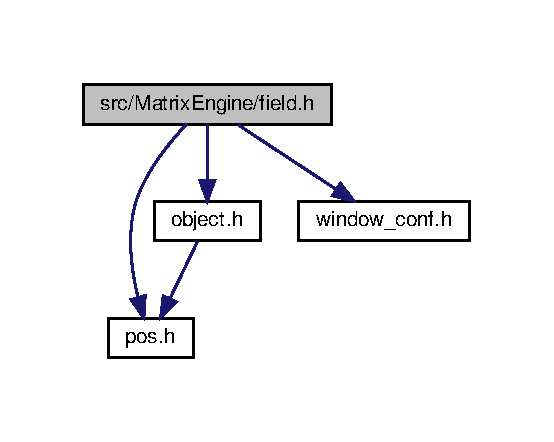
\includegraphics[width=266pt]{field_8h__incl}
\end{center}
\end{figure}
This graph shows which files directly or indirectly include this file\+:
\nopagebreak
\begin{figure}[H]
\begin{center}
\leavevmode
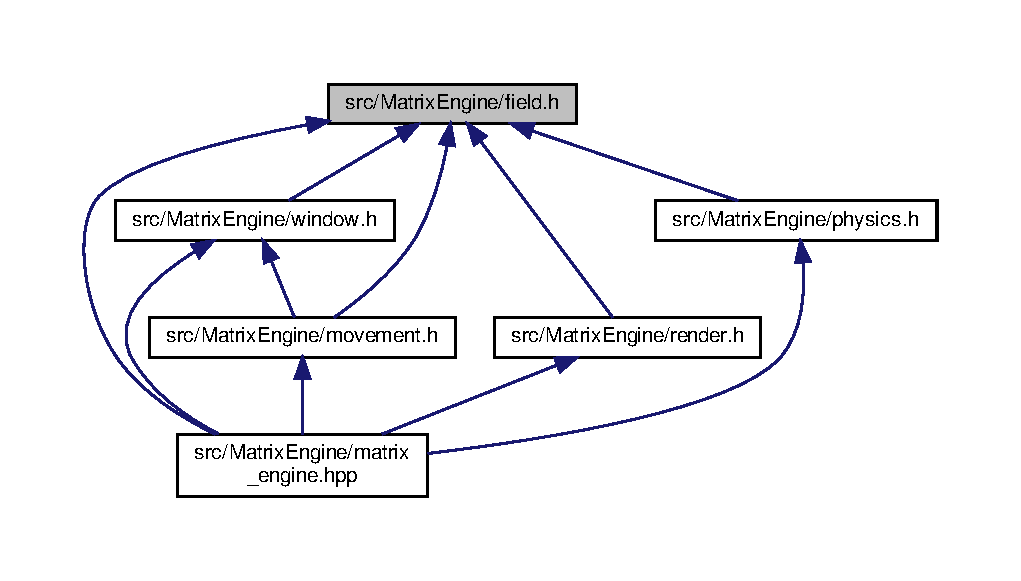
\includegraphics[width=350pt]{field_8h__dep__incl}
\end{center}
\end{figure}
\subsection*{Classes}
\begin{DoxyCompactItemize}
\item 
class \hyperlink{classfield}{field}
\begin{DoxyCompactList}\small\item\em Entire playground of the scene. \end{DoxyCompactList}\end{DoxyCompactItemize}

\hypertarget{led__matrix_8hpp}{}\section{src/\+Matrix\+Engine/led\+\_\+matrix.hpp File Reference}
\label{led__matrix_8hpp}\index{src/\+Matrix\+Engine/led\+\_\+matrix.\+hpp@{src/\+Matrix\+Engine/led\+\_\+matrix.\+hpp}}
{\ttfamily \#include \char`\"{}hwlib.\+hpp\char`\"{}}\newline
Include dependency graph for led\+\_\+matrix.\+hpp\+:
\nopagebreak
\begin{figure}[H]
\begin{center}
\leavevmode
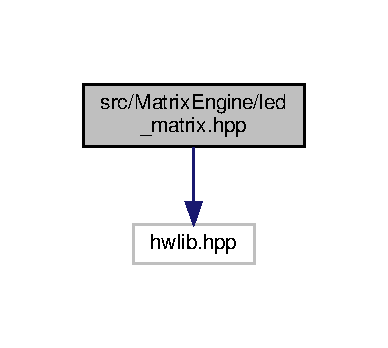
\includegraphics[width=186pt]{led__matrix_8hpp__incl}
\end{center}
\end{figure}
This graph shows which files directly or indirectly include this file\+:
\nopagebreak
\begin{figure}[H]
\begin{center}
\leavevmode
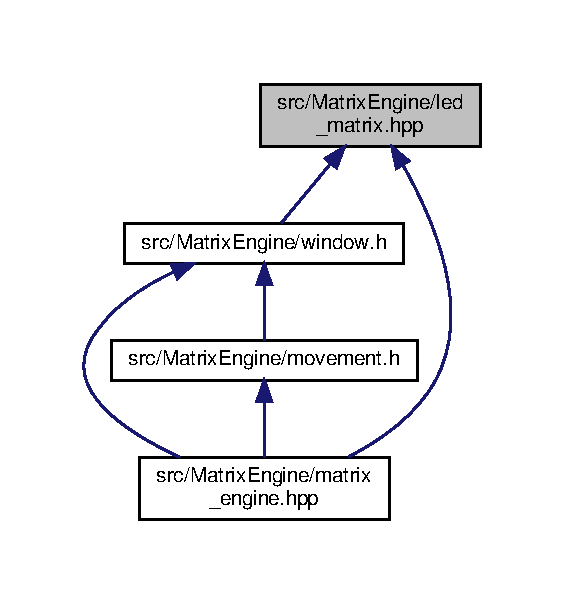
\includegraphics[width=271pt]{led__matrix_8hpp__dep__incl}
\end{center}
\end{figure}
\subsection*{Classes}
\begin{DoxyCompactItemize}
\item 
class \hyperlink{classled__matrix}{led\+\_\+matrix}
\begin{DoxyCompactList}\small\item\em Interface for the M\+H7219 led matrix chip. \end{DoxyCompactList}\end{DoxyCompactItemize}

\hypertarget{movement_8h}{}\section{src/\+Matrix\+Engine/movement.h File Reference}
\label{movement_8h}\index{src/\+Matrix\+Engine/movement.\+h@{src/\+Matrix\+Engine/movement.\+h}}
{\ttfamily \#include \char`\"{}object.\+h\char`\"{}}\newline
{\ttfamily \#include \char`\"{}field.\+h\char`\"{}}\newline
{\ttfamily \#include \char`\"{}window.\+h\char`\"{}}\newline
{\ttfamily \#include \char`\"{}window\+\_\+conf.\+h\char`\"{}}\newline
Include dependency graph for movement.\+h\+:
\nopagebreak
\begin{figure}[H]
\begin{center}
\leavevmode
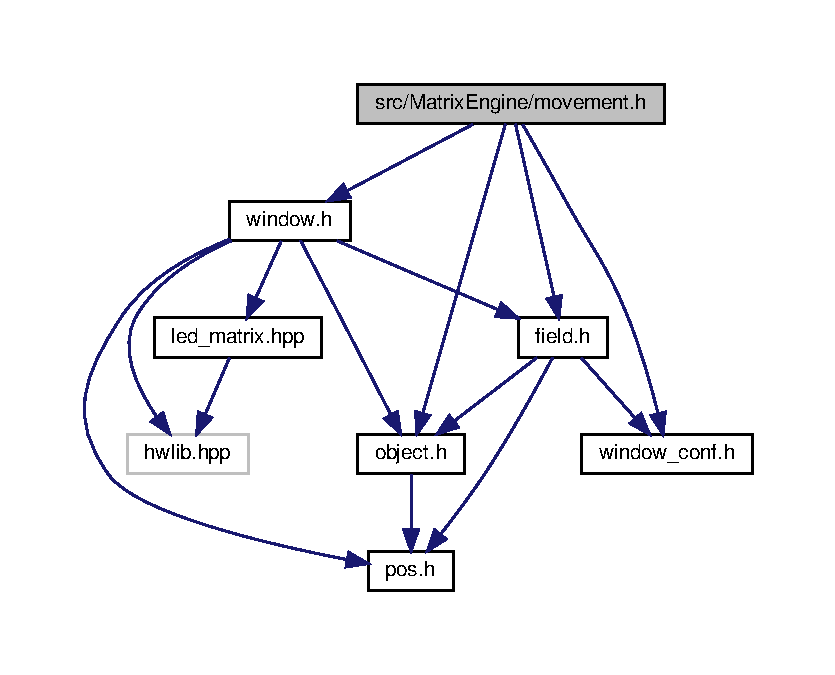
\includegraphics[width=350pt]{movement_8h__incl}
\end{center}
\end{figure}
This graph shows which files directly or indirectly include this file\+:
\nopagebreak
\begin{figure}[H]
\begin{center}
\leavevmode
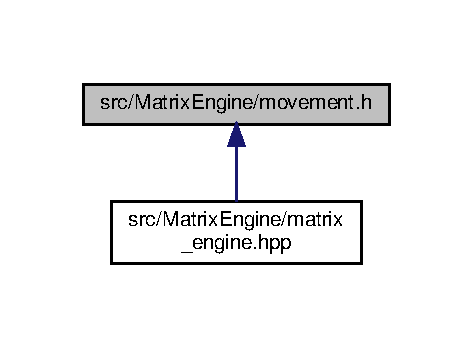
\includegraphics[width=227pt]{movement_8h__dep__incl}
\end{center}
\end{figure}
\subsection*{Functions}
\begin{DoxyCompactItemize}
\item 
void \hyperlink{movement_8h_a09c373da69e4b1875fb45d4fa03a62a3}{make\+\_\+move} (const char \&move, \hyperlink{classentity}{entity} \&speler, \hyperlink{classfield}{field} \&veld)
\item 
void \hyperlink{movement_8h_affe859be9e4907f125894c7cd59220aa}{make\+\_\+move} (const char \&move, \hyperlink{classwindow}{window} \&camera, \hyperlink{classfield}{field} \&veld)
\end{DoxyCompactItemize}


\subsection{Function Documentation}
\mbox{\Hypertarget{movement_8h_a09c373da69e4b1875fb45d4fa03a62a3}\label{movement_8h_a09c373da69e4b1875fb45d4fa03a62a3}} 
\index{movement.\+h@{movement.\+h}!make\+\_\+move@{make\+\_\+move}}
\index{make\+\_\+move@{make\+\_\+move}!movement.\+h@{movement.\+h}}
\subsubsection{\texorpdfstring{make\+\_\+move()}{make\_move()}\hspace{0.1cm}{\footnotesize\ttfamily [1/2]}}
{\footnotesize\ttfamily void make\+\_\+move (\begin{DoxyParamCaption}\item[{const char \&}]{move,  }\item[{\hyperlink{classentity}{entity} \&}]{speler,  }\item[{\hyperlink{classfield}{field} \&}]{veld }\end{DoxyParamCaption})}

\textbackslash{} brief generates next position of entity \textbackslash{} details Generate next position of an entity on input value d (down) u (up) l (left) r (right) Object only moves when his next position is equal to air. \mbox{\Hypertarget{movement_8h_affe859be9e4907f125894c7cd59220aa}\label{movement_8h_affe859be9e4907f125894c7cd59220aa}} 
\index{movement.\+h@{movement.\+h}!make\+\_\+move@{make\+\_\+move}}
\index{make\+\_\+move@{make\+\_\+move}!movement.\+h@{movement.\+h}}
\subsubsection{\texorpdfstring{make\+\_\+move()}{make\_move()}\hspace{0.1cm}{\footnotesize\ttfamily [2/2]}}
{\footnotesize\ttfamily void make\+\_\+move (\begin{DoxyParamCaption}\item[{const char \&}]{move,  }\item[{\hyperlink{classwindow}{window} \&}]{camera,  }\item[{\hyperlink{classfield}{field} \&}]{veld }\end{DoxyParamCaption})}

\textbackslash{} brief generates next position of camera \textbackslash{} details Generate next position of an entity on input value d (down) u (up) l (left) r (right) Object only moves when his next position is equal to air. 
\hypertarget{object_8h}{}\section{src/\+Matrix\+Engine/object.h File Reference}
\label{object_8h}\index{src/\+Matrix\+Engine/object.\+h@{src/\+Matrix\+Engine/object.\+h}}
{\ttfamily \#include \char`\"{}pos.\+h\char`\"{}}\newline
Include dependency graph for object.\+h\+:
\nopagebreak
\begin{figure}[H]
\begin{center}
\leavevmode
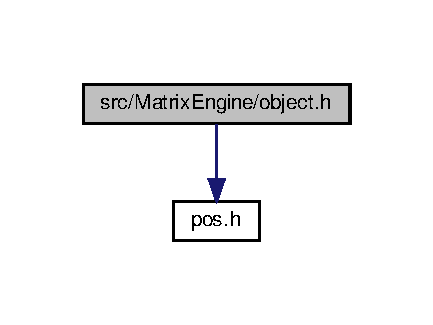
\includegraphics[width=208pt]{object_8h__incl}
\end{center}
\end{figure}
This graph shows which files directly or indirectly include this file\+:
\nopagebreak
\begin{figure}[H]
\begin{center}
\leavevmode
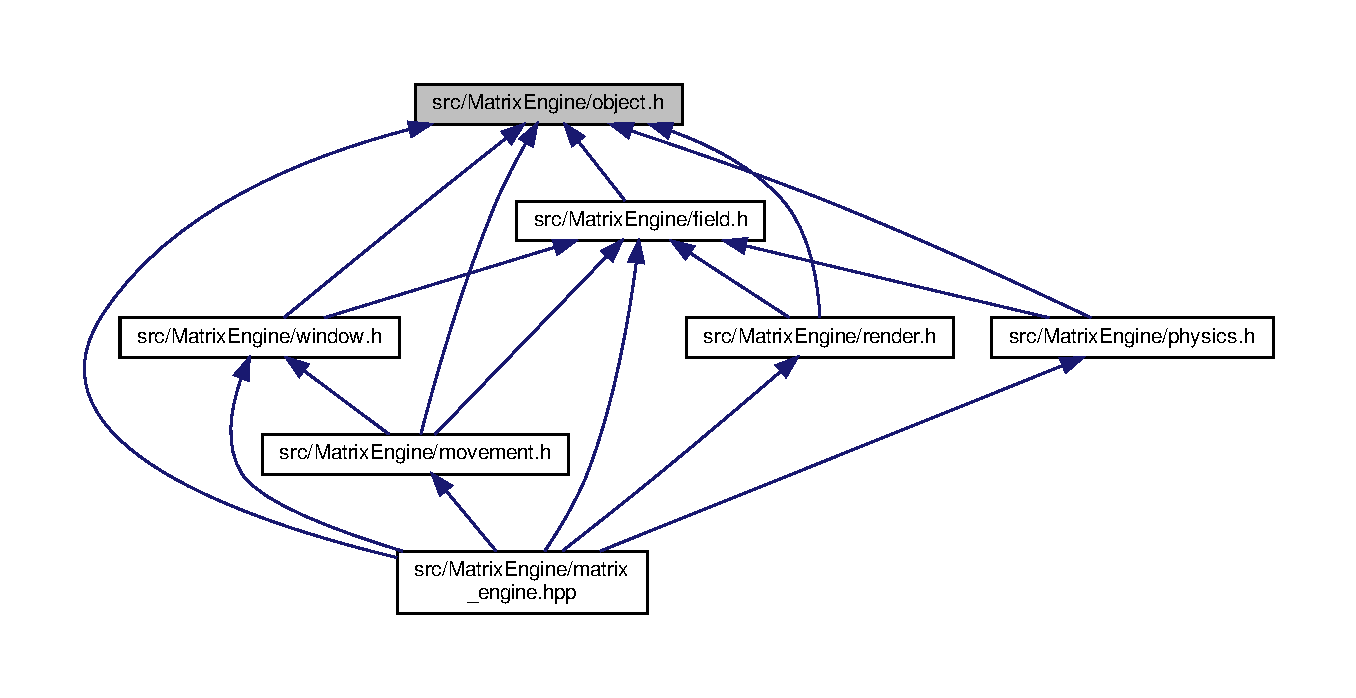
\includegraphics[width=350pt]{object_8h__dep__incl}
\end{center}
\end{figure}
\subsection*{Classes}
\begin{DoxyCompactItemize}
\item 
class \hyperlink{classobject}{object}
\begin{DoxyCompactList}\small\item\em A void object with a position. \end{DoxyCompactList}\item 
class \hyperlink{classentity}{entity}
\begin{DoxyCompactList}\small\item\em A visable entity. \end{DoxyCompactList}\item 
class \hyperlink{classobstacle}{obstacle}
\begin{DoxyCompactList}\small\item\em Solid Object with a start end point. \end{DoxyCompactList}\item 
class \hyperlink{classplayer}{player}
\begin{DoxyCompactList}\small\item\em Inherited class solely made for the frog jump demo. \end{DoxyCompactList}\end{DoxyCompactItemize}

\hypertarget{physics_8h}{}\section{src/\+Matrix\+Engine/physics.h File Reference}
\label{physics_8h}\index{src/\+Matrix\+Engine/physics.\+h@{src/\+Matrix\+Engine/physics.\+h}}
{\ttfamily \#include \char`\"{}field.\+h\char`\"{}}\newline
{\ttfamily \#include \char`\"{}object.\+h\char`\"{}}\newline
{\ttfamily \#include \char`\"{}window\+\_\+conf.\+h\char`\"{}}\newline
Include dependency graph for physics.\+h\+:
\nopagebreak
\begin{figure}[H]
\begin{center}
\leavevmode
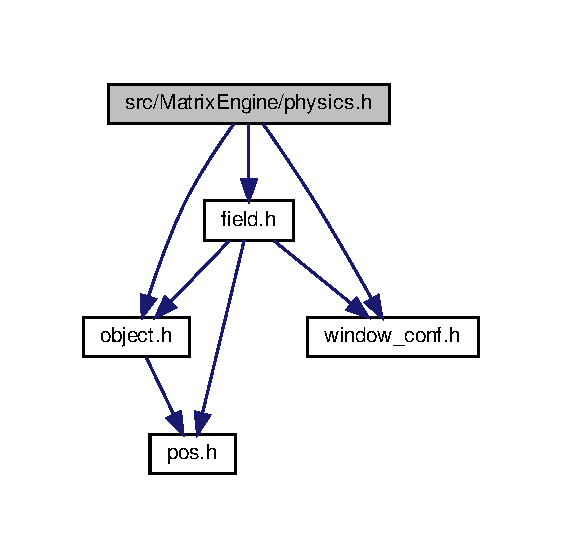
\includegraphics[width=270pt]{physics_8h__incl}
\end{center}
\end{figure}
This graph shows which files directly or indirectly include this file\+:
\nopagebreak
\begin{figure}[H]
\begin{center}
\leavevmode
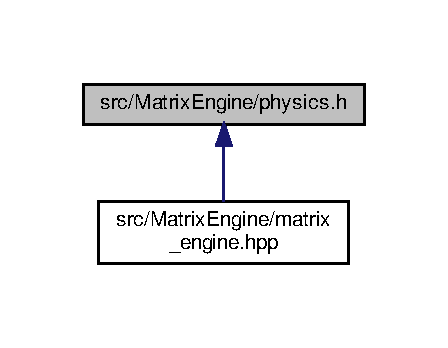
\includegraphics[width=215pt]{physics_8h__dep__incl}
\end{center}
\end{figure}
\subsection*{Classes}
\begin{DoxyCompactItemize}
\item 
class \hyperlink{classphysbox}{physbox}
\begin{DoxyCompactList}\small\item\em Physics engine. \end{DoxyCompactList}\end{DoxyCompactItemize}

\hypertarget{pos_8h}{}\section{src/\+Matrix\+Engine/pos.h File Reference}
\label{pos_8h}\index{src/\+Matrix\+Engine/pos.\+h@{src/\+Matrix\+Engine/pos.\+h}}
This graph shows which files directly or indirectly include this file\+:
\nopagebreak
\begin{figure}[H]
\begin{center}
\leavevmode
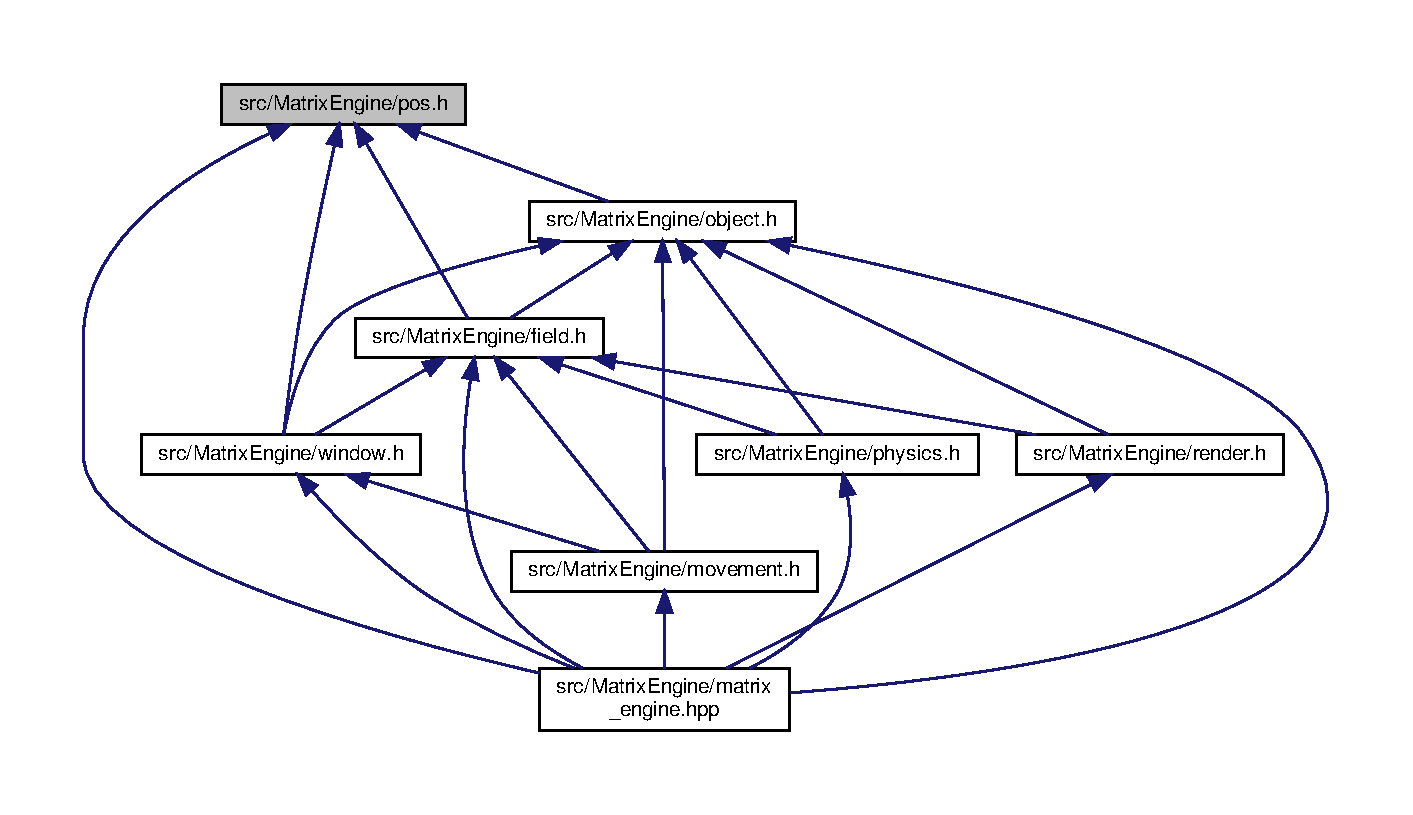
\includegraphics[width=350pt]{pos_8h__dep__incl}
\end{center}
\end{figure}
\subsection*{Classes}
\begin{DoxyCompactItemize}
\item 
class \hyperlink{classxyz}{xyz}
\begin{DoxyCompactList}\small\item\em 3D postion A\+DT \end{DoxyCompactList}\item 
class \hyperlink{classxy}{xy}
\begin{DoxyCompactList}\small\item\em 2D postion A\+DT \end{DoxyCompactList}\item 
class \hyperlink{classposTouch}{pos\+Touch}
\begin{DoxyCompactList}\small\item\em Collision A\+DT. \end{DoxyCompactList}\end{DoxyCompactItemize}

\hypertarget{window_8h}{}\section{src/\+Matrix\+Engine/window.h File Reference}
\label{window_8h}\index{src/\+Matrix\+Engine/window.\+h@{src/\+Matrix\+Engine/window.\+h}}
{\ttfamily \#include \char`\"{}pos.\+h\char`\"{}}\newline
{\ttfamily \#include \char`\"{}field.\+h\char`\"{}}\newline
{\ttfamily \#include \char`\"{}object.\+h\char`\"{}}\newline
{\ttfamily \#include \char`\"{}led\+\_\+matrix.\+hpp\char`\"{}}\newline
{\ttfamily \#include \char`\"{}hwlib.\+hpp\char`\"{}}\newline
Include dependency graph for window.\+h\+:
\nopagebreak
\begin{figure}[H]
\begin{center}
\leavevmode
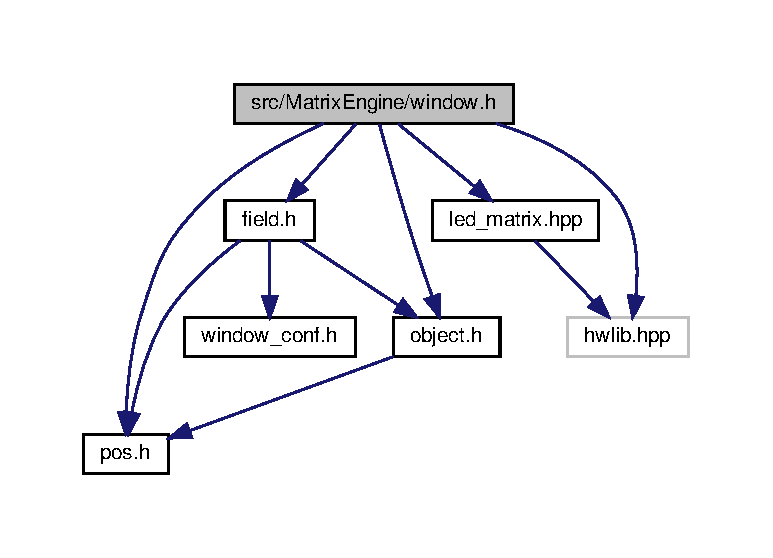
\includegraphics[width=350pt]{window_8h__incl}
\end{center}
\end{figure}
This graph shows which files directly or indirectly include this file\+:
\nopagebreak
\begin{figure}[H]
\begin{center}
\leavevmode
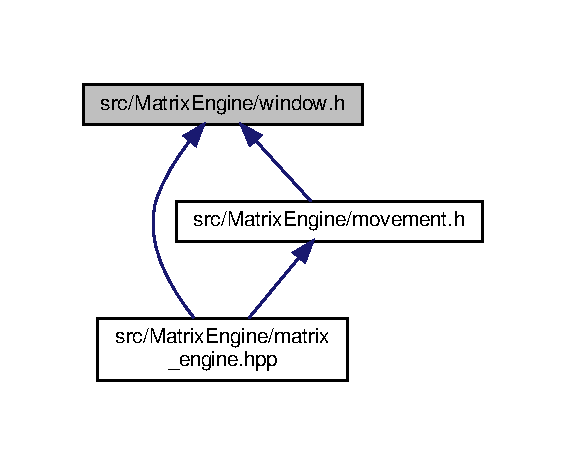
\includegraphics[width=272pt]{window_8h__dep__incl}
\end{center}
\end{figure}
\subsection*{Classes}
\begin{DoxyCompactItemize}
\item 
class \hyperlink{classwindow}{window}
\begin{DoxyCompactList}\small\item\em Renders all data within the sizes and positions. \end{DoxyCompactList}\end{DoxyCompactItemize}

%--- End generated contents ---

% Index
\backmatter
\newpage
\phantomsection
\clearemptydoublepage
\addcontentsline{toc}{chapter}{Index}
\printindex

\end{document}
